\chapter{Apresentação e Análise dos Resultados}
\label{cap:resultados}

Este capítulo apresenta e discute os resultados quantitativos da síntese empírica do método USARP, obtidos a partir da reanálise da base consolidada no nível do respondente e interpretados em conjunto com as evidências reportadas nos quatro estudos primários. Conforme detalhado na metodologia, a matriz quantitativa reúne as respostas dos estudos que aplicaram o instrumento comum de levantamento, a saber, o estudo de caso na indústria de \citeonline{marques2022}, o estudo de caso acadêmico de \citeonline{fiori2022} e o estudo de caso na indústria de \citeonline{simoes2022usarp}, além das demais coortes que aplicaram o mesmo instrumento. O estudo pioneiro de \citeonline{oliveirajr2020}, por anteceder a versão do método em cartas e adotar grupo focal com \textit{Grounded Theory}, não compõe a matriz quantitativa e é retomado na análise qualitativa. A organização das seções acompanha a sequência analítica da metodologia: caracterização da amostra, estatística descritiva e normalidade, estrutura de correlação, adequação amostral, análise de componentes principais, detecção de observações atípicas, segmentação não supervisionada e comparações entre grupos. A análise qualitativa temática e a discussão integrada são apresentadas nas seções finais deste capítulo (a partir da Seção \ref{sec:res-qualitativa}).

\section{Composição da Amostra Consolidada}
\label{sec:res-amostra}

A base consolidada reuniu 68 registros provenientes das aplicações do instrumento comum. Identificou-se um único valor ausente entre as dez variáveis-núcleo (item de guia de prototipação, em respondente do contexto industrial), tratado conforme descrito na metodologia, de impacto desprezível (um valor em 680 células). Após as verificações de consistência e a classificação completa por contexto e coorte, a amostra analítica empregada nas etapas multivariadas compreendeu 67 respondentes. Desses, 56 pertencem ao contexto acadêmico e 11 ao contexto industrial, distribuídos em seis coortes, conforme a Figura \ref{fig:composicao-amostra} e a Tabela \ref{tab:composicao-amostra}.

A predominância de respondentes acadêmicos reflete a natureza das aplicações disponíveis: enquanto os estudos industriais envolveram equipes de desenvolvimento de porte reduzido, com sete respondentes em \citeonline{marques2022} e poucos respondentes em \citeonline{simoes2022usarp}, as aplicações acadêmicas reuniram turmas inteiras de Engenharia de Software organizadas em equipes, como em \citeonline{fiori2022}. Essa assimetria amostral, com subamostra industrial pequena, é considerada explicitamente na interpretação das comparações entre contextos (Seção \ref{sec:res-comparacoes}).

Cabe esclarecer a procedência das coortes posteriores à última publicação sobre o método. O instrumento não foi aplicado apenas nas ocasiões reportadas nos estudos primários. Em especial, a coorte de 2025-1 é composta por integrantes do LUDI (Laboratório de Pesquisa e Desenvolvimento para Usabilidade, Diversidade e Inclusão), laboratório ao qual o método está vinculado, que utilizaram o USARP em projetos desenvolvidos no próprio laboratório. Esses participantes atuaram em diferentes funções, como analista de requisitos, agilista, desenvolvedor, projetista de UI/UX e profissional de garantia da qualidade. As respostas coletadas foram incorporadas a um registro unificado. Por se tratar de um ambiente universitário de pesquisa e desenvolvimento, essa coorte foi classificada como pertencente ao contexto acadêmico, enquanto a classificação de indústria foi reservada às equipes de empresas parceiras.

\begin{figure}[h!]
    \centering
    \caption{Composição da amostra consolidada por coorte e contexto}
    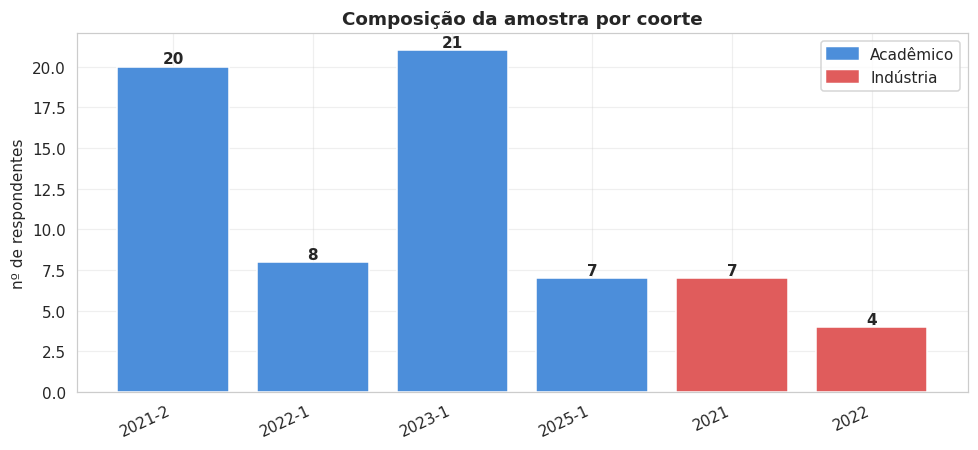
\includegraphics[width=0.85\textwidth]{figuras/composicao_amostra_coorte.png}
    \label{fig:composicao-amostra}
    \Fonte{Elaborada pelo autor (2026).}
\end{figure}

\begin{table}[h!]
    \centering
    \captionsetup{width=15cm}
    \caption{Distribuição dos respondentes por contexto e coorte}
    \label{tab:composicao-amostra}
    \IBGEtab{}{
        \begin{tabular}{llc}
            \toprule
            \textbf{Contexto} & \textbf{Coorte} & \textbf{n} \\
            \midrule \midrule
            Acadêmico & 2021-2 & 20 \\
            Acadêmico & 2022-1 & 8 \\
            Acadêmico & 2023-1 & 21 \\
            Acadêmico & 2025-1 & 7 \\
            Indústria & 2021 & 7 \\
            Indústria & 2022 & 4 \\
            \midrule
            \multicolumn{2}{l}{\textbf{Total}} & \textbf{67} \\
            \bottomrule
        \end{tabular}
        }{
            \Fonte{Elaborada pelo autor (2026).}
            }
        \end{table}
        

\section{Caracterização Descritiva e Efeito de Teto}
\label{sec:res-descritiva}

A Tabela \ref{tab:descritivas} resume as estatísticas descritivas das dez variáveis-núcleo e a Figura \ref{fig:distribuicao-itens} apresenta a distribuição das respostas por item. Os quatro itens de percepção geral, avaliados em escala de 1 a 5, concentram-se em valores elevados, com médias entre 4,48 e 4,70. Os seis itens referentes ao conteúdo das cartas, avaliados em escala de 1 a 6, situam-se ainda mais próximos do extremo superior, com médias entre 5,52 e 5,90. O item de contexto do mecanismo de usabilidade (cartas amarelas) apresenta a maior concentração, com média 5,90 e mediana 6.

\begin{table}[h!]
\centering
\captionsetup{width=15cm}
\caption{Estatísticas descritivas das variáveis-núcleo}
\label{tab:descritivas}
\IBGEtab{}{
\begin{tabular}{lccccccc}
\toprule
\textbf{Item} & \textbf{Média} & \textbf{DP} & \textbf{Mín} & \textbf{Q1} & \textbf{Mediana} & \textbf{Q3} & \textbf{Máx} \\
\midrule \midrule
Desempenho       & 4,48 & 0,70 & 3 & 4 & 5 & 5 & 5 \\
Produtividade    & 4,51 & 0,75 & 2 & 4 & 5 & 5 & 5 \\
Eficácia         & 4,52 & 0,70 & 2 & 4 & 5 & 5 & 5 \\
Utilidade        & 4,70 & 0,52 & 3 & 4 & 5 & 5 & 5 \\
Desc. mecanismo  & 5,69 & 0,58 & 3 & 5 & 6 & 6 & 6 \\
Contexto mecan.  & 5,90 & 0,43 & 3 & 6 & 6 & 6 & 6 \\
Questão requis.  & 5,78 & 0,71 & 1 & 6 & 6 & 6 & 6 \\
Guia requisito   & 5,67 & 0,70 & 2 & 6 & 6 & 6 & 6 \\
Questão prot.    & 5,67 & 0,59 & 3 & 5 & 6 & 6 & 6 \\
Guia prototip.   & 5,52 & 0,70 & 2 & 5 & 6 & 6 & 6 \\
\bottomrule
\end{tabular}
}{
\Fonte{Elaborada pelo autor (2026).}
}
\end{table}

\begin{figure}[h!]
    \centering
    \caption{Distribuição das respostas por item}
    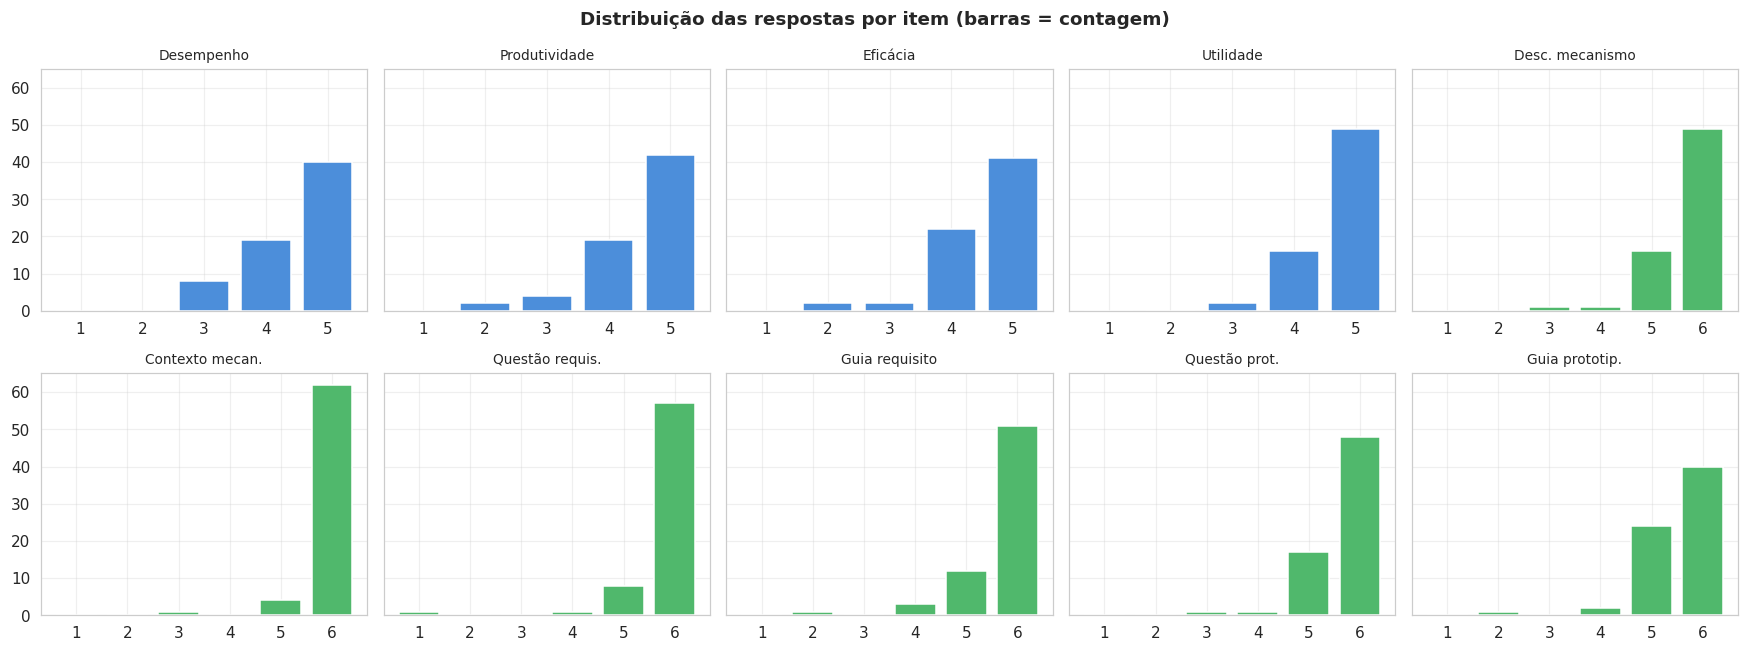
\includegraphics[width=\textwidth]{figuras/distribuicao_respostas_itens.png}
    \label{fig:distribuicao-itens}
    \Fonte{Elaborada pelo autor (2026).}
\end{figure}

\FloatBarrier

Esse padrão evidencia um acentuado efeito de teto, isto é, a saturação das respostas nos níveis superiores das escalas. O fenômeno é coerente com os resultados individuais dos estudos primários, nos quais a percepção sobre o método foi consistentemente positiva: em \citeonline{marques2022}, todos os respondentes manifestaram concordância quanto à utilidade e à efetividade do método; em \citeonline{fiori2022}, a maioria dos estudantes concordou parcial ou totalmente com as afirmações de desempenho, produtividade, eficácia e utilidade; e em \citeonline{simoes2022usarp}, os participantes igualmente concordaram quanto ao potencial do método para a elicitação de requisitos de usabilidade. A base consolidada, portanto, expressa de forma agregada a avaliação favorável já observada isoladamente em cada cenário.

As Tabelas \ref{tab:medias-contexto} e \ref{tab:medias-coorte} detalham as médias por contexto e por coorte. As diferenças de média entre os contextos são pequenas em todos os itens, e a variação entre coortes também é modesta, antecipando o quadro de convergência confirmado nas análises inferenciais (Seção \ref{sec:res-comparacoes}).

\begin{table}[h!]
\centering
\captionsetup{width=15cm}
\caption{Médias das variáveis-núcleo por contexto}
\label{tab:medias-contexto}
\IBGEtab{}{
\resizebox{\textwidth}{!}{%
\begin{tabular}{lcccccccccc}
\toprule
\textbf{Contexto} & \textbf{Desemp.} & \textbf{Produt.} & \textbf{Eficácia} & \textbf{Utilid.} & \textbf{Desc. mec.} & \textbf{Cont. mec.} & \textbf{Q. requis.} & \textbf{Guia req.} & \textbf{Q. prot.} & \textbf{Guia prot.} \\
\midrule \midrule
Acadêmico & 4,48 & 4,50 & 4,46 & 4,70 & 5,71 & 5,96 & 5,77 & 5,64 & 5,64 & 5,50 \\
Indústria & 4,45 & 4,55 & 4,82 & 4,73 & 5,55 & 5,55 & 5,82 & 5,82 & 5,82 & 5,64 \\
\bottomrule
\end{tabular}%
}
}{
\Fonte{Elaborada pelo autor (2026).}
}
\end{table}

\begin{table}[h!]
\centering
\captionsetup{width=15cm}
\caption{Médias das variáveis-núcleo por coorte}
\label{tab:medias-coorte}
\IBGEtab{}{
\resizebox{\textwidth}{!}{%
\begin{tabular}{lcccccccccc}
\toprule
\textbf{Coorte} & \textbf{Desemp.} & \textbf{Produt.} & \textbf{Eficácia} & \textbf{Utilid.} & \textbf{Desc. mec.} & \textbf{Cont. mec.} & \textbf{Q. requis.} & \textbf{Guia req.} & \textbf{Q. prot.} & \textbf{Guia prot.} \\
\midrule \midrule
2021    & 4,71 & 4,86 & 4,86 & 4,86 & 5,86 & 5,86 & 5,86 & 5,71 & 5,86 & 5,71 \\
2021-2  & 4,35 & 4,30 & 4,40 & 4,65 & 5,50 & 6,00 & 5,80 & 5,50 & 5,60 & 5,20 \\
2022    & 4,00 & 4,00 & 4,75 & 4,50 & 5,00 & 5,00 & 5,75 & 6,00 & 5,75 & 5,50 \\
2022-1  & 4,50 & 5,00 & 4,75 & 4,88 & 5,88 & 6,00 & 5,88 & 5,75 & 5,88 & 5,75 \\
2023-1  & 4,52 & 4,38 & 4,33 & 4,62 & 5,81 & 6,00 & 5,86 & 5,90 & 5,57 & 5,67 \\
2025-1  & 4,71 & 4,86 & 4,71 & 4,86 & 5,86 & 5,71 & 5,29 & 5,14 & 5,71 & 5,57 \\
\bottomrule
\end{tabular}%
}
}{
\Fonte{Elaborada pelo autor (2026).}
}
\end{table}

\FloatBarrier

Quanto ao site de apoio, dos 67 respondentes, 15 declararam ter utilizado o recurso. Entre esses, as médias dos cinco aspectos avaliados foram 4,73 para aprendizagem, 4,60 para relembrar, 4,53 para interpretar, 4,40 para aplicação e 4,33 para \textit{brainstorming}, em escala de 1 a 5. Como discutido na metodologia, essas variáveis foram tratadas apenas de forma descritiva, dada a ausência estrutural de respostas para quem não utilizou o recurso.

A Tabela \ref{tab:shapiro} apresenta o teste de normalidade de Shapiro-Wilk e a assimetria de cada item. Todos os dez itens rejeitam a hipótese de normalidade (p < 0,001), e a assimetria é negativa em todos eles, o que confirma quantitativamente o efeito de teto. Esse diagnóstico fundamenta as escolhas inferenciais adotadas nas seções seguintes: a correlação de postos de Spearman e os testes não-paramétricos de Kruskal-Wallis e Mann-Whitney nas comparações entre grupos \cite{field2018}.

\begin{table}[h!]
\centering
\captionsetup{width=15cm}
\caption{Teste de normalidade de Shapiro-Wilk e assimetria por item}
\label{tab:shapiro}
\IBGEtab{}{
\begin{tabular}{lccc}
\toprule
\textbf{Item} & \textbf{Assimetria} & \textbf{Estatística W} & \textbf{Conclusão} \\
\midrule \midrule
Desempenho       & -0,97 & 0,705 & não-normal \\
Produtividade    & -1,57 & 0,677 & não-normal \\
Eficácia         & -1,65 & 0,667 & não-normal \\
Utilidade        & -1,50 & 0,590 & não-normal \\
Desc. mecanismo  & -2,15 & 0,571 & não-normal \\
Contexto mecan.  & -5,16 & 0,261 & não-normal \\
Questão requis.  & -4,94 & 0,346 & não-normal \\
Guia requisito   & -2,85 & 0,524 & não-normal \\
Questão prot.    & -2,05 & 0,585 & não-normal \\
Guia prototip.   & -2,18 & 0,641 & não-normal \\
\bottomrule
\end{tabular}
}{
\Fonte{Elaborada pelo autor (2026). Nota: todos os itens apresentaram p < 0,001.}
}
\end{table}

\FloatBarrier

\section{Estrutura de Correlação entre as Variáveis}
\label{sec:res-correlacao}

A Figura \ref{fig:correlacao} apresenta a matriz de correlação de Spearman entre as dez variáveis-núcleo. A matriz foi estimada sobre a amostra completa, isto é, sobre os 67 respondentes, sem separação por contexto ou por coorte, conforme justificado na Seção \ref{sec:correlacao}: esta etapa é diagnóstica e prepara a PCA, que também é ajustada sobre a matriz completa, e a estimação de uma matriz de dez variáveis em subgrupos pequenos, como a subamostra industrial de onze respondentes, produziria coeficientes instáveis. As diferenças entre contextos e coortes são investigadas na Seção \ref{sec:res-comparacoes}, por testes apropriados ao tamanho da amostra. A correlação média, em módulo, fora da diagonal, é de 0,225, e a correlação máxima observada é de 0,572. As associações mais fortes ocorrem dentro de cada bloco de itens. No bloco de percepção geral, destacam-se as correlações entre utilidade e produtividade ($\rho = 0{,}56$) e entre utilidade e desempenho ($\rho = 0{,}42$). No bloco das cartas, sobressaem as correlações entre questão de prototipação e guia de prototipação ($\rho = 0{,}57$), entre descrição do mecanismo e questão de prototipação ($\rho = 0{,}52$) e entre questão e guia de requisitos ($\rho = 0{,}47$). As correlações entre os dois blocos são, em geral, fracas, e o item de contexto do mecanismo mostra-se praticamente independente dos demais, inclusive com associação ligeiramente negativa com o guia de requisitos ($\rho = -0{,}16$). Esse padrão de blocos relativamente coesos e fracamente associados entre si antecipa a estrutura latente revelada pela análise de componentes principais.

\begin{figure}[h!]
    \centering
    \caption{Matriz de correlação de Spearman entre as variáveis-núcleo}
    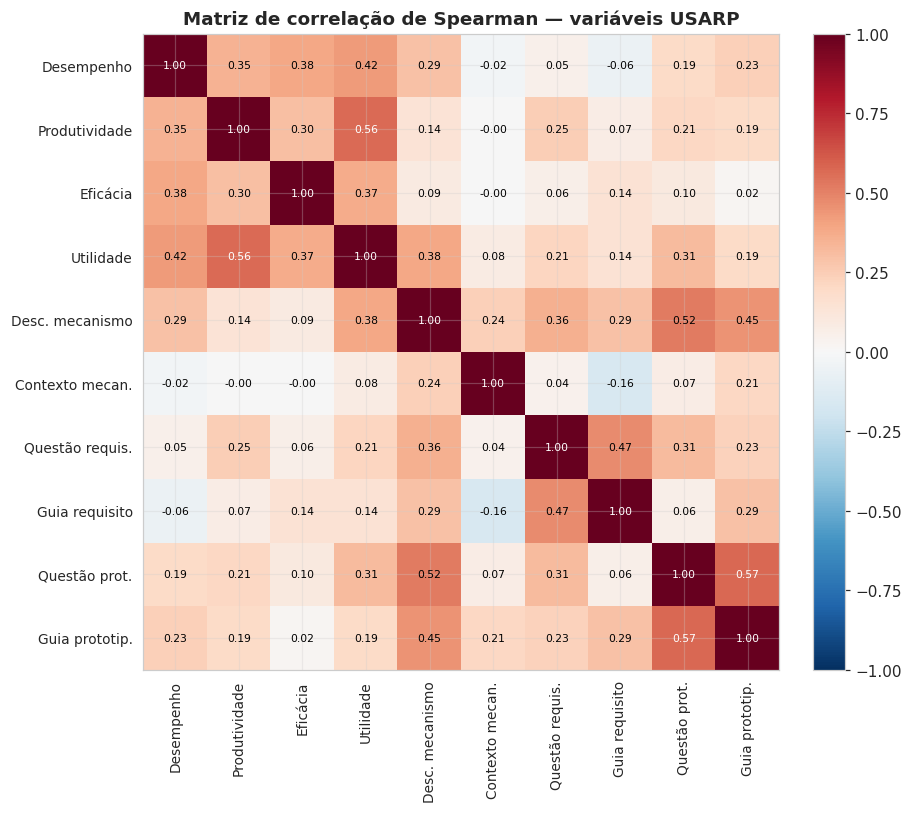
\includegraphics[width=0.8\textwidth]{figuras/correlacao_spearman.png}
    \label{fig:correlacao}
    \Fonte{Elaborada pelo autor (2026).}
\end{figure}

\FloatBarrier

\section{Adequação Amostral à Análise de Componentes Principais}
\label{sec:res-adequacao}

Os diagnósticos de adequação amostral apresentaram resultados divergentes, o que orienta a interpretação subsequente. O teste de esfericidade de Bartlett rejeitou fortemente a hipótese de ausência de correlação ($\chi^2 = 238{,}6$; $\mathrm{gl} = 45$; $p = 3{,}54 \times 10^{-28}$), indicando que existe estrutura a ser extraída \cite{bartlett1950}. A medida de Kaiser-Meyer-Olkin, por sua vez, resultou em $\mathrm{KMO} = 0{,}461$, valor classificado como inaceitável segundo os limiares usuais \cite{kaiser1974,field2018}. Esse contraste é coerente com a natureza dos dados: em amostras pequenas e com forte efeito de teto, diversas variáveis saturam no valor máximo e reduzem a variância compartilhável, deprimindo o KMO. Por essa razão, e em consonância com \citeonline{hair2019}, a análise de componentes principais é empregada neste trabalho como técnica exploratória e descritiva, voltada a resumir a variabilidade e a identificar agrupamentos de itens, e não como análise fatorial confirmatória. Essa ressalva é mantida em toda a interpretação dos componentes.

\section{Análise de Componentes Principais}
\label{sec:res-pca}

A Tabela \ref{tab:autovalores} apresenta os autovalores e a variância explicada por componente, e a Figura \ref{fig:scree} exibe o \textit{scree plot} e a variância acumulada. Pelo critério de Kaiser (autovalor superior a um), retêm-se três componentes, que acumulam 64,4\% da variância \cite{kaiser1960}. Os limiares de variância acumulada de 80\%, 90\% e 95\% são atingidos, respectivamente, com cinco, sete e oito componentes. O erro de reconstrução (Figura \ref{fig:mse}) decresce de forma suave, sem um cotovelo abrupto: três componentes recompõem os dados com erro quadrático médio de aproximadamente 0,356, e cinco componentes reduzem esse erro para cerca de 0,199. A ausência de um ponto de inflexão nítido é típica de dados com efeito de teto e correlações moderadas, nos quais a informação se distribui por várias dimensões, o que reforça o caráter exploratório da análise. Conforme a metodologia, adotaram-se três componentes para a interpretação substantiva e cinco componentes para as análises que dependem de mais dimensões, como a segmentação e a matriz de dispersão.

\begin{table}[h!]
\centering
\captionsetup{width=15cm}
\caption{Autovalores e variância explicada por componente principal}
\label{tab:autovalores}
\IBGEtab{}{
\begin{tabular}{lccc}
\toprule
\textbf{Componente} & \textbf{Autovalor} & \textbf{Variância (\%)} & \textbf{Acumulada (\%)} \\
\midrule \midrule
PC1  & 3,242 & 31,94 & 31,94 \\
PC2  & 1,913 & 18,85 & 50,78 \\
PC3  & 1,383 & 13,62 & 64,40 \\
PC4  & 0,835 & 8,22  & 72,63 \\
PC5  & 0,756 & 7,45  & 80,07 \\
PC6  & 0,645 & 6,35  & 86,43 \\
PC7  & 0,569 & 5,61  & 92,03 \\
PC8  & 0,420 & 4,14  & 96,17 \\
PC9  & 0,286 & 2,82  & 98,99 \\
PC10 & 0,103 & 1,01  & 100,00 \\
\bottomrule
\end{tabular}
}{
\Fonte{Elaborada pelo autor (2026). Nota: três componentes retidos pelo critério de Kaiser; cinco componentes atingem 80\% da variância.}
}
\end{table}

\begin{figure}[h!]
    \centering
    \caption{Escolha do número de componentes: scree plot e variância acumulada}
    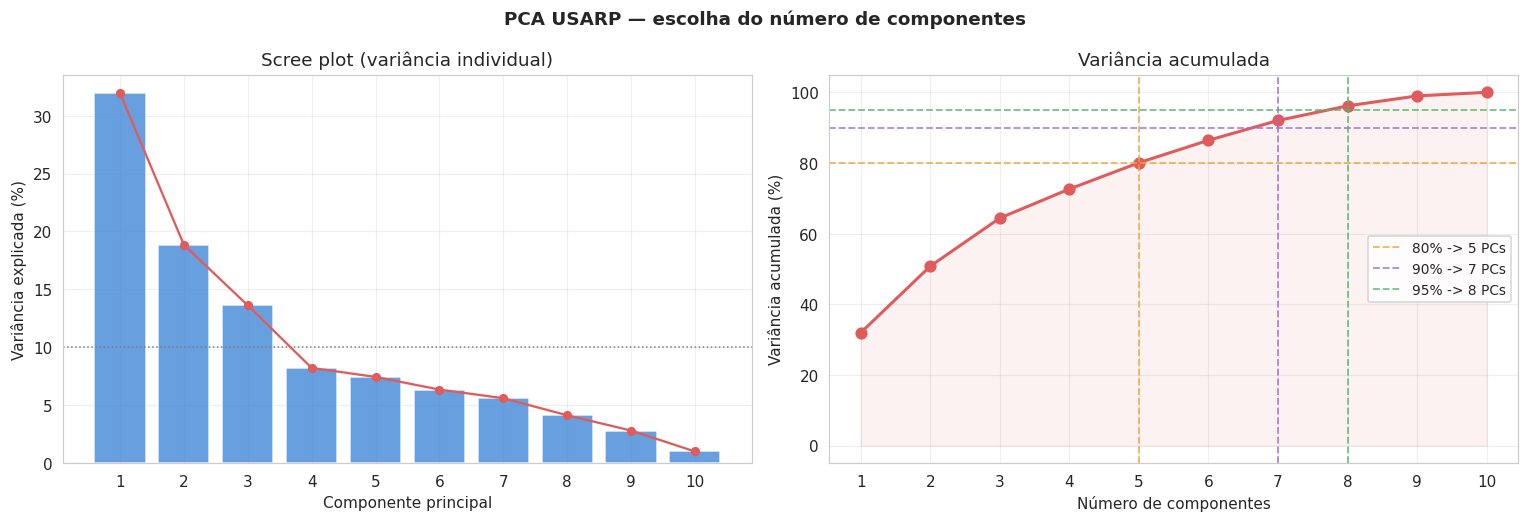
\includegraphics[width=\textwidth]{figuras/pca_scree_variancia.png}
    \label{fig:scree}
    \Fonte{Elaborada pelo autor (2026).}
\end{figure}

\begin{figure}[h!]
    \centering
    \caption{Erro de reconstrução em função do número de componentes}
    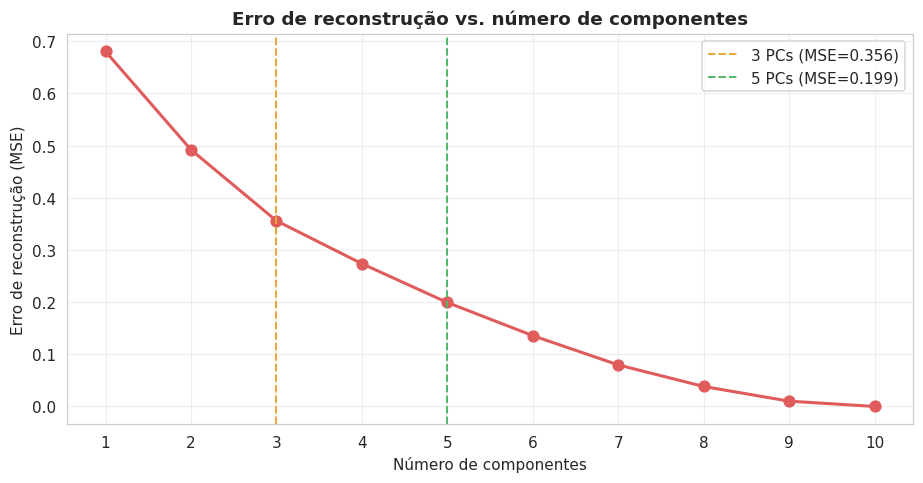
\includegraphics[width=0.8\textwidth]{figuras/erro_reconstrucao.png}
    \label{fig:mse}
    \Fonte{Elaborada pelo autor (2026).}
\end{figure}

\FloatBarrier

A Tabela \ref{tab:loadings} e a Figura \ref{fig:loadings} apresentam as cargas fatoriais das cinco primeiras componentes, que orientam a interpretação substantiva.

\begin{table}[h!]
\centering
\captionsetup{width=15cm}
\caption{Cargas fatoriais (loadings) das cinco primeiras componentes}
\label{tab:loadings}
\IBGEtab{}{
\begin{tabular}{lccccc}
\toprule
\textbf{Variável} & \textbf{PC1} & \textbf{PC2} & \textbf{PC3} & \textbf{PC4} & \textbf{PC5} \\
\midrule \midrule
Desempenho       & 0,534 & -0,442 & -0,030 & -0,007 & 0,640 \\
Produtividade    & 0,605 & -0,421 & -0,229 & -0,244 & -0,394 \\
Eficácia         & 0,539 & -0,470 & -0,228 & -0,246 & 0,063 \\
Utilidade        & 0,728 & -0,313 & -0,020 & -0,171 & -0,119 \\
Desc. mecanismo  & 0,644 & 0,364  & 0,522  & -0,058 & 0,113 \\
Contexto mecan.  & 0,285 & 0,138  & 0,829  & -0,273 & -0,023 \\
Questão requis.  & 0,383 & 0,764  & -0,236 & -0,291 & -0,046 \\
Guia requisito   & 0,375 & 0,677  & -0,506 & -0,159 & 0,169 \\
Questão prot.    & 0,720 & 0,072  & 0,052  & 0,436  & -0,338 \\
Guia prototip.   & 0,685 & 0,147  & -0,056 & 0,554  & 0,117 \\
\bottomrule
\end{tabular}
}{
\Fonte{Elaborada pelo autor (2026).}
}
\end{table}

\begin{figure}[h!]
    \centering
    \caption{Mapa de calor das cargas fatoriais das cinco primeiras componentes}
    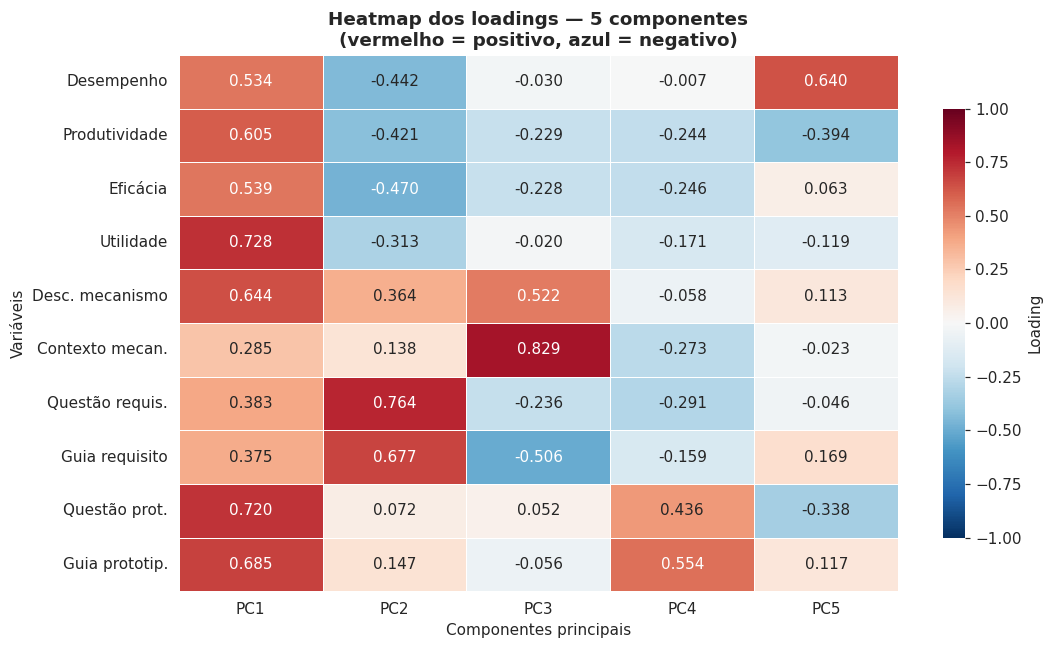
\includegraphics[width=0.85\textwidth]{figuras/pca_loadings_heatmap.png}
    \label{fig:loadings}
    \Fonte{Elaborada pelo autor (2026).}
\end{figure}

\FloatBarrier

A primeira componente (31,9\% da variância) apresenta cargas positivas em todas as variáveis, com maior peso em utilidade (0,728), questão de prototipação (0,720), guia de prototipação (0,685) e descrição do mecanismo (0,644). Trata-se, portanto, de um eixo de percepção positiva geral do método: respondentes que avaliam bem um aspecto tendem a avaliar bem os demais. A segunda componente (18,8\%) opõe os itens das cartas de requisitos, questão de requisitos (0,764) e guia de requisitos (0,677), aos itens de percepção geral, eficácia ($-0{,}470$), desempenho ($-0{,}442$) e produtividade ($-0{,}421$), configurando um contraste entre a utilidade percebida das cartas de requisitos e a percepção de eficiência operacional do método. A terceira componente (13,6\%) é dominada pelo contexto do mecanismo (0,829) e pela descrição do mecanismo (0,522), em oposição ao guia de requisitos ($-0{,}506$), capturando a dimensão das cartas de mecanismo, ligada à contextualização. As componentes seguintes têm peso reduzido: a quarta associa-se à prototipação (guia 0,554 e questão 0,436) e a quinta a um contraste interno do bloco de percepção, liderado pelo desempenho (0,640).

As Figuras \ref{fig:biplot12}, \ref{fig:biplot13} e \ref{fig:biplot23} apresentam os \textit{biplots} das combinações das três primeiras componentes, e as Figuras \ref{fig:proj12}, \ref{fig:proj13} e \ref{fig:proj23} exibem as projeções dos respondentes por contexto e por coorte. A Figura \ref{fig:proj3d} apresenta a projeção tridimensional e a Figura \ref{fig:scatter} a matriz de dispersão das três primeiras componentes.

Como esses gráficos concentram boa parte da interpretação da PCA, convém explicitar sua leitura. Um \textit{biplot} sobrepõe, em um mesmo plano formado por duas componentes, dois elementos de naturezas distintas. Os \textbf{pontos} representam os respondentes, posicionados segundo seus escores nas duas componentes do plano e coloridos conforme o contexto de aplicação; dois pontos próximos indicam participantes com perfis de resposta semelhantes. Os \textbf{vetores} representam as dez variáveis originais, projetadas no mesmo plano a partir de suas cargas fatoriais. A leitura dos vetores segue três convenções: a \textbf{direção} indica o sentido em que a variável cresce, de modo que respondentes situados ao longo dela tendem a atribuir notas mais altas naquele item; o \textbf{comprimento} indica o quanto a variável é bem representada naquele plano, sendo os vetores mais longos os que mais contribuem para as componentes exibidas; e o \textbf{ângulo} entre dois vetores aproxima a associação entre as variáveis, pois ângulos pequenos sugerem itens que variam em conjunto, ângulos próximos de noventa graus sugerem itens praticamente independentes e ângulos próximos de cento e oitenta graus sugerem itens que variam em sentidos opostos.

Nos três biplots, todos os vetores das variáveis projetam-se sobre o lado positivo de PC1, o que confirma visualmente o eixo de percepção positiva geral: independentemente do plano observado, as setas apontam para a direita, de modo que escores altos em PC1 correspondem a avaliações favoráveis em todos os itens. A nuvem de respondentes concentra-se majoritariamente nesse lado positivo, com poucos casos deslocados para a esquerda, padrão coerente com o efeito de teto e com a predominância de percepções favoráveis. No plano PC1 e PC2 (Figura \ref{fig:biplot12}), os vetores de questão e guia de requisitos apontam para cima e formam entre si um ângulo pequeno, enquanto utilidade, produtividade, desempenho e eficácia apontam para baixo, materializando o contraste identificado nas cargas: a valorização das cartas de requisitos varia em sentido oposto à percepção de eficiência operacional. Nos planos que incluem PC3 (Figuras \ref{fig:biplot13} e \ref{fig:biplot23}), o contexto e a descrição do mecanismo destacam-se na direção vertical, isolando a dimensão das cartas de mecanismo das demais variáveis. Quanto ao contexto de aplicação, os pontos acadêmicos e de indústria sobrepõem-se amplamente nos três planos, sem formar agrupamentos distintos, com os respondentes de indústria situados dentro da nuvem acadêmica. Não há, assim, indício visual de que o contexto module o perfil de resposta.

\begin{figure}[h!]
    \centering
    \caption{Biplot das componentes PC1 e PC2, por contexto}
    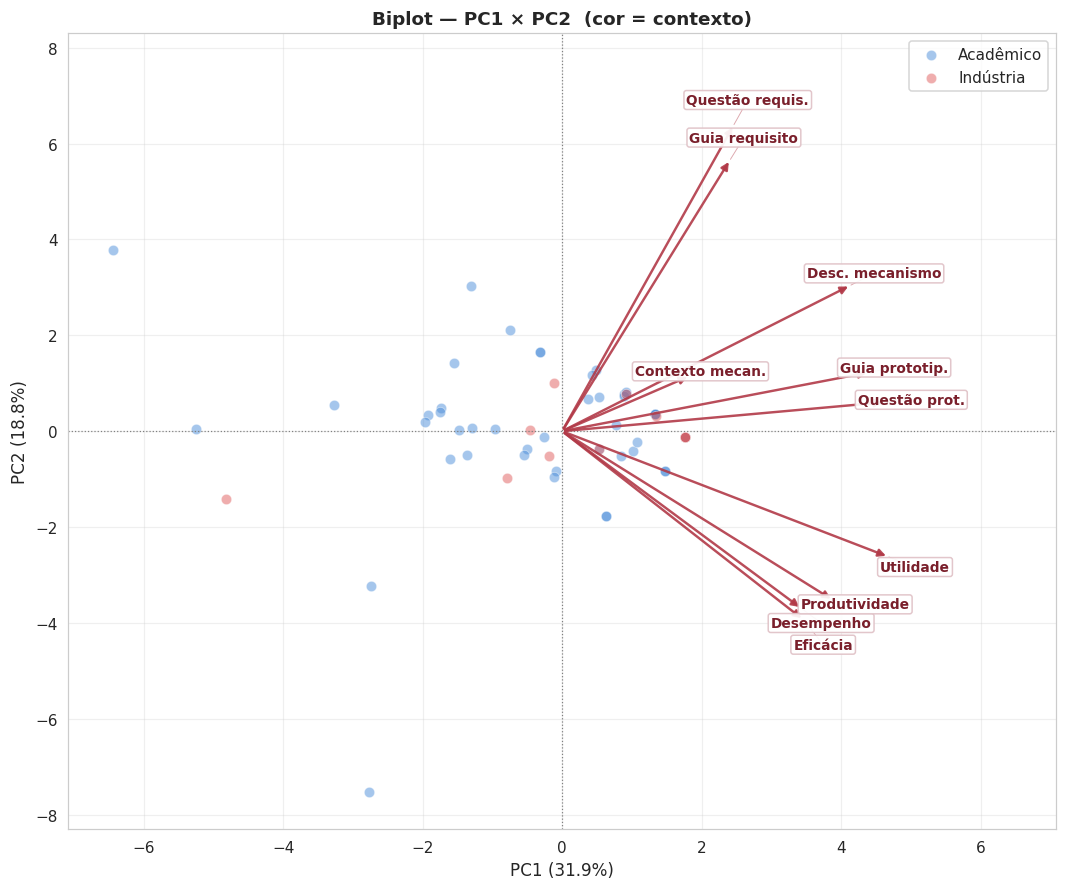
\includegraphics[width=0.8\textwidth]{figuras/biplot_pc1_pc2.png}
    \label{fig:biplot12}
    \Fonte{Elaborada pelo autor (2026).}
\end{figure}

\begin{figure}[h!]
    \centering
    \caption{Biplot das componentes PC1 e PC3, por contexto}
    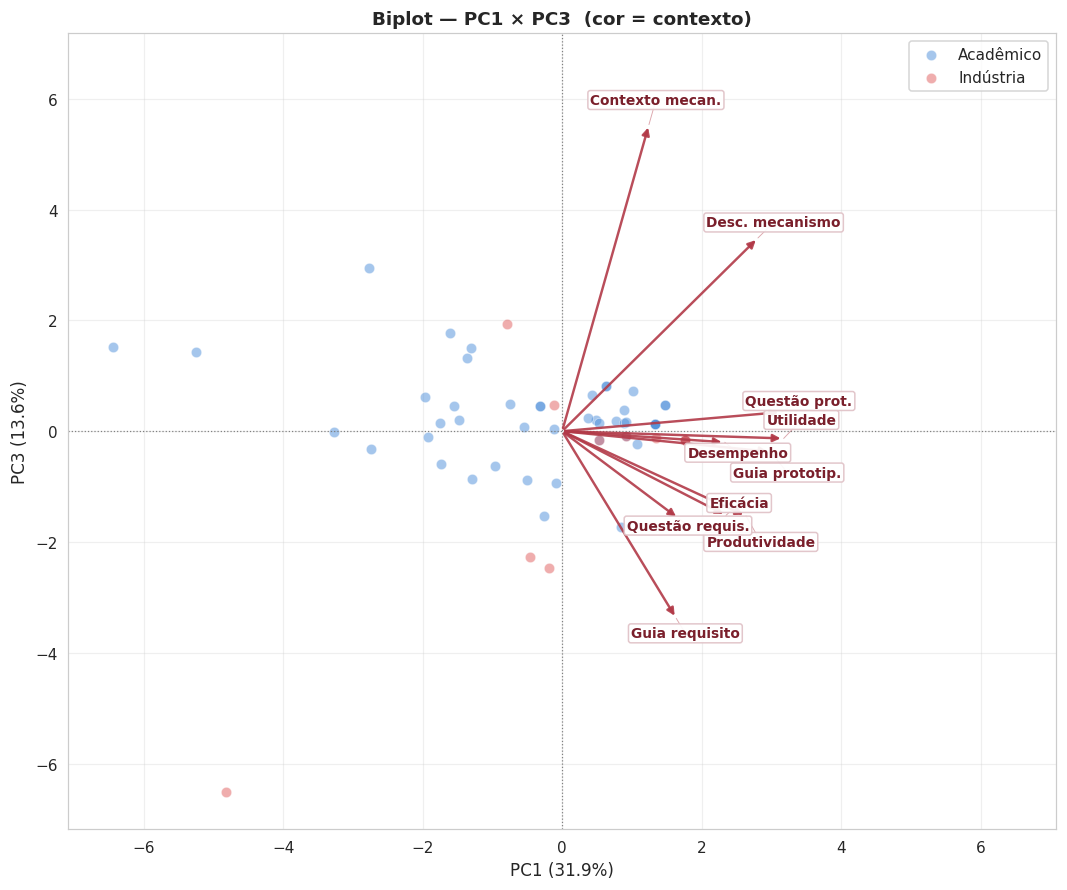
\includegraphics[width=0.8\textwidth]{figuras/biplot_pc1_pc3.png}
    \label{fig:biplot13}
    \Fonte{Elaborada pelo autor (2026).}
\end{figure}

\begin{figure}[h!]
    \centering
    \caption{Biplot das componentes PC2 e PC3, por contexto}
    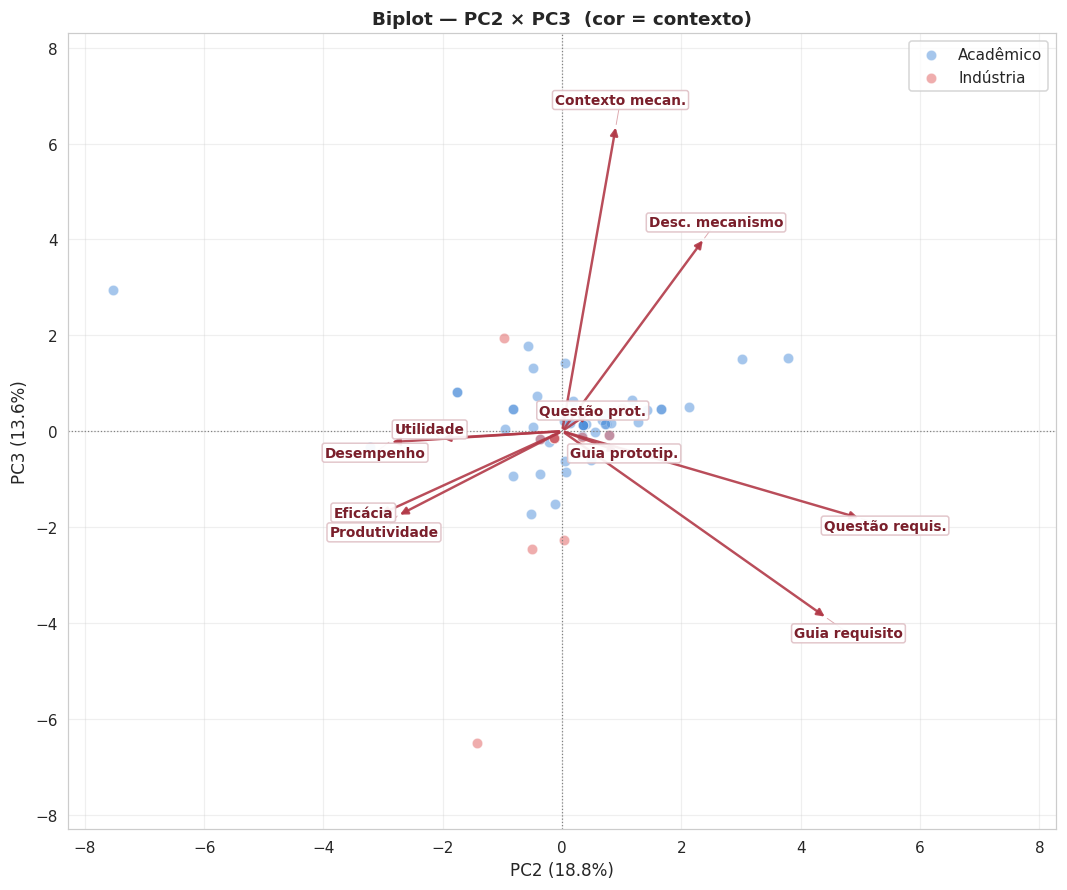
\includegraphics[width=0.8\textwidth]{figuras/biplot_pc2_pc3.png}
    \label{fig:biplot23}
    \Fonte{Elaborada pelo autor (2026).}
\end{figure}

\begin{figure}[h!]
    \centering
    \caption{Projeção dos respondentes nas componentes PC1 e PC2, por contexto e por coorte}
    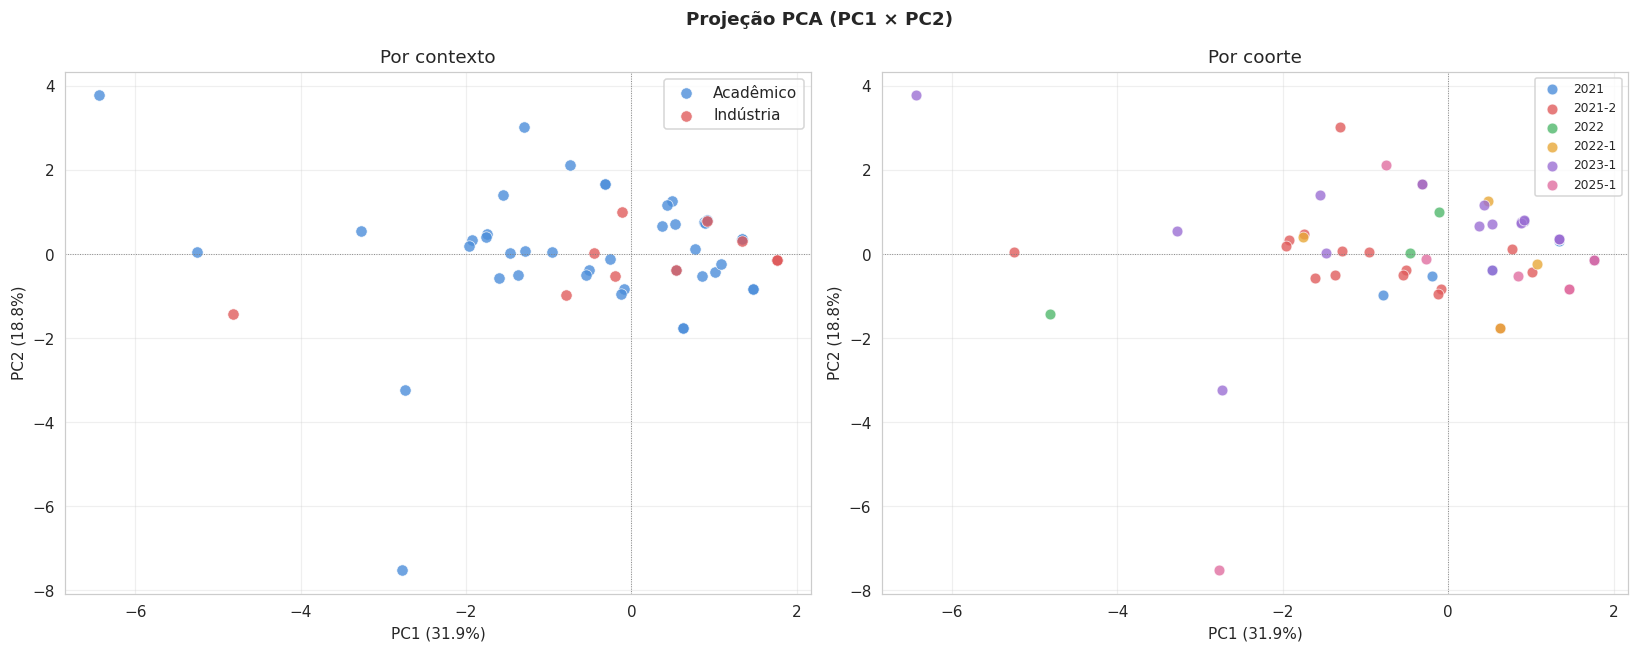
\includegraphics[width=\textwidth]{figuras/projecao_pca_pc1_pc2.png}
    \label{fig:proj12}
    \Fonte{Elaborada pelo autor (2026).}
\end{figure}

\begin{figure}[h!]
    \centering
    \caption{Projeção dos respondentes nas componentes PC1 e PC3, por contexto e por coorte}
    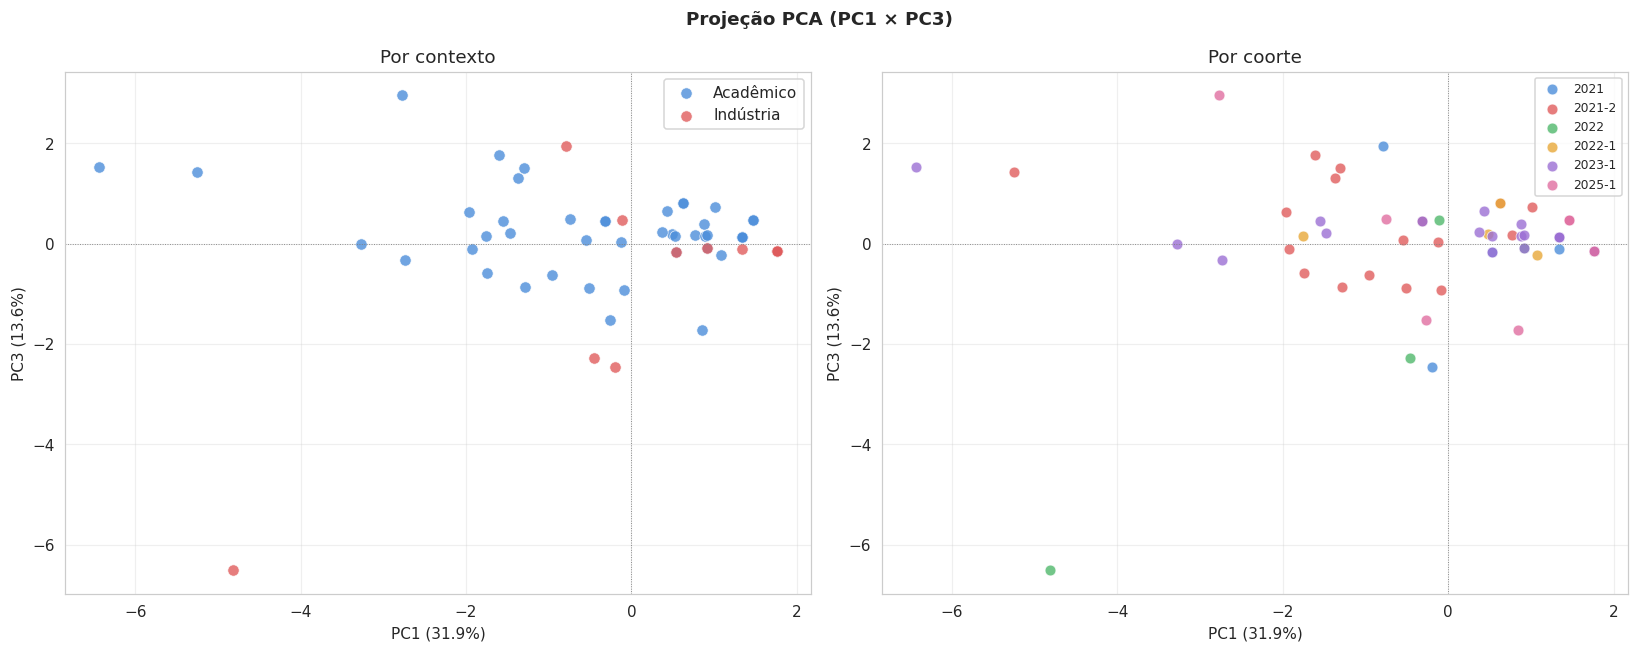
\includegraphics[width=\textwidth]{figuras/projecao_pca_pc1_pc3.png}
    \label{fig:proj13}
    \Fonte{Elaborada pelo autor (2026).}
\end{figure}

\begin{figure}[h!]
    \centering
    \caption{Projeção dos respondentes nas componentes PC2 e PC3, por contexto e por coorte}
    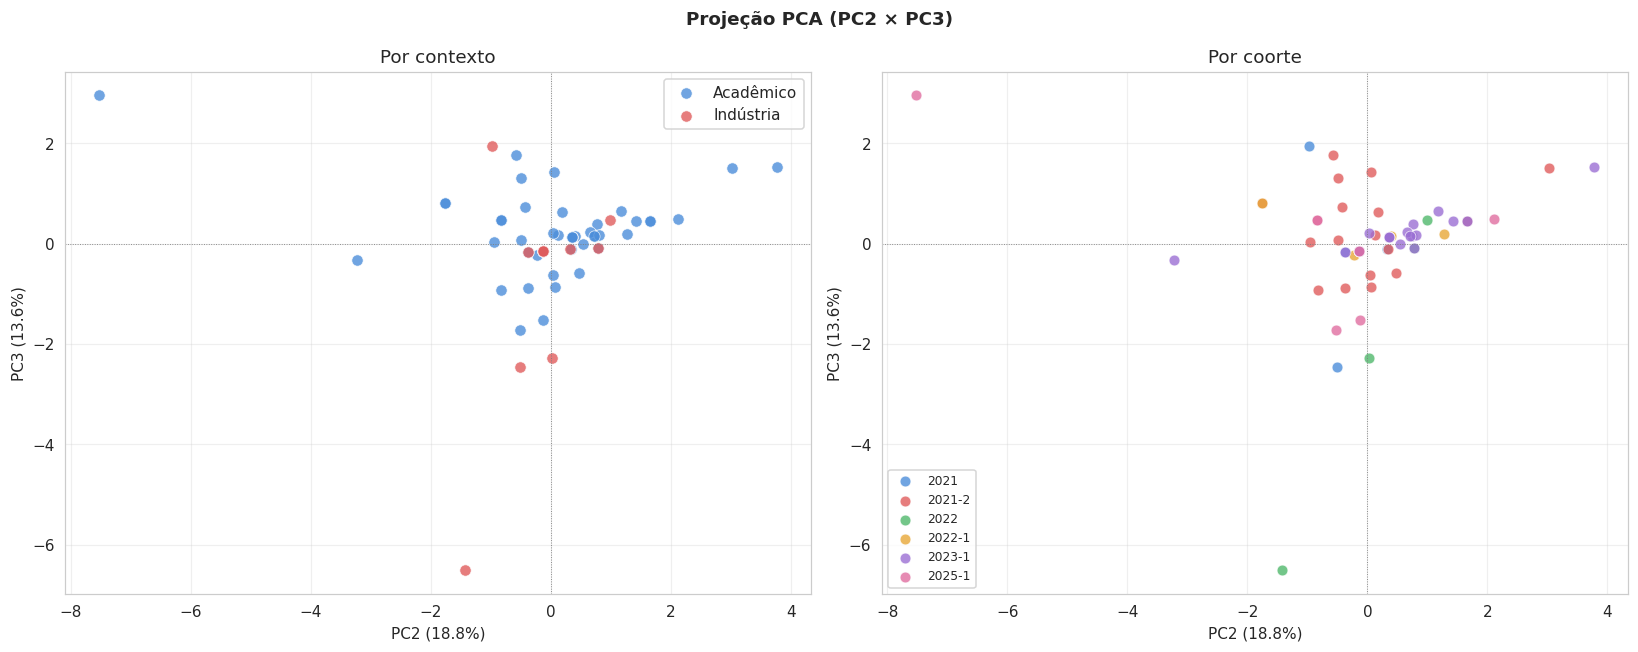
\includegraphics[width=\textwidth]{figuras/projecao_pca_pc2_pc3.png}
    \label{fig:proj23}
    \Fonte{Elaborada pelo autor (2026).}
\end{figure}

\begin{figure}[h!]
    \centering
    \caption{Projeção tridimensional das três primeiras componentes, por contexto}
    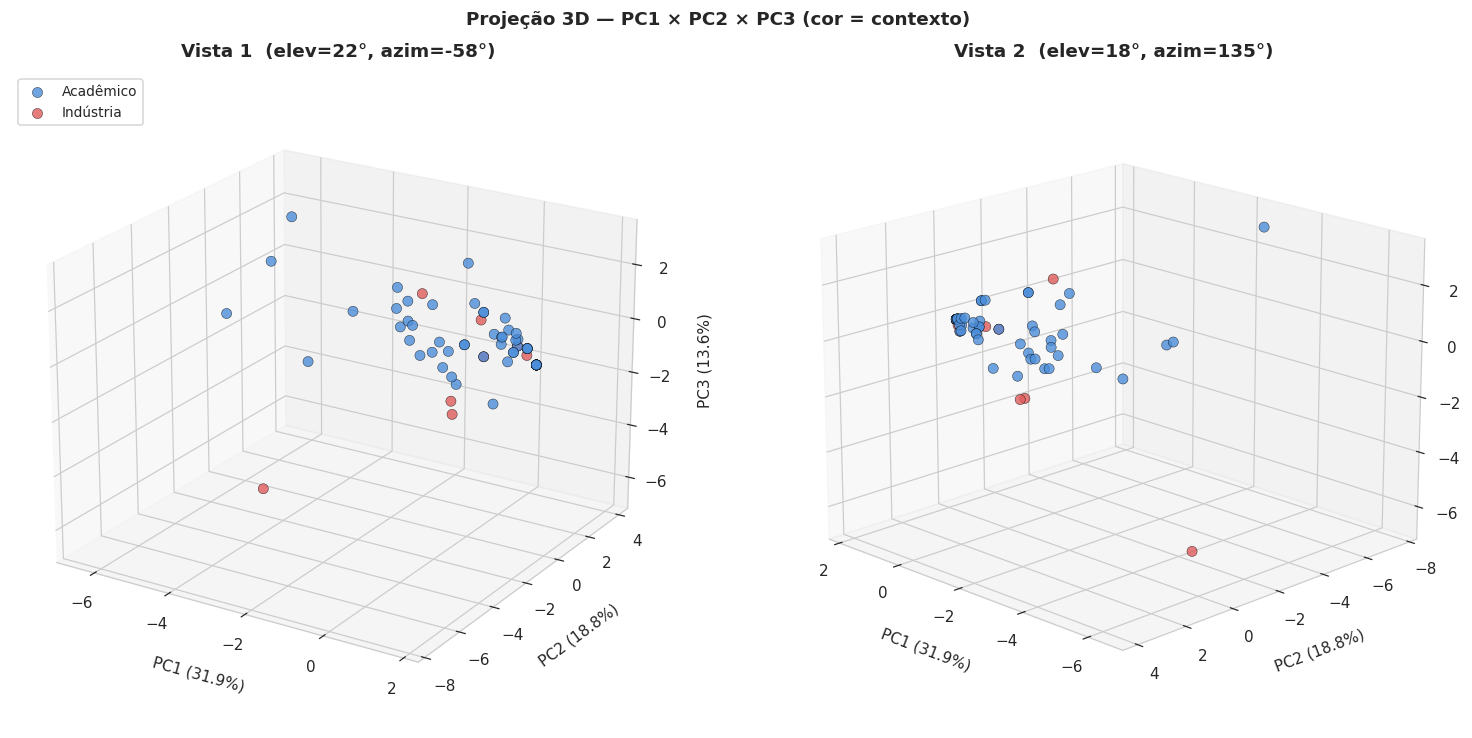
\includegraphics[width=\textwidth]{figuras/projecao_3d_pca.png}
    \label{fig:proj3d}
    \Fonte{Elaborada pelo autor (2026).}
\end{figure}

\begin{figure}[h!]
    \centering
    \caption{Matriz de dispersão das três primeiras componentes principais}
    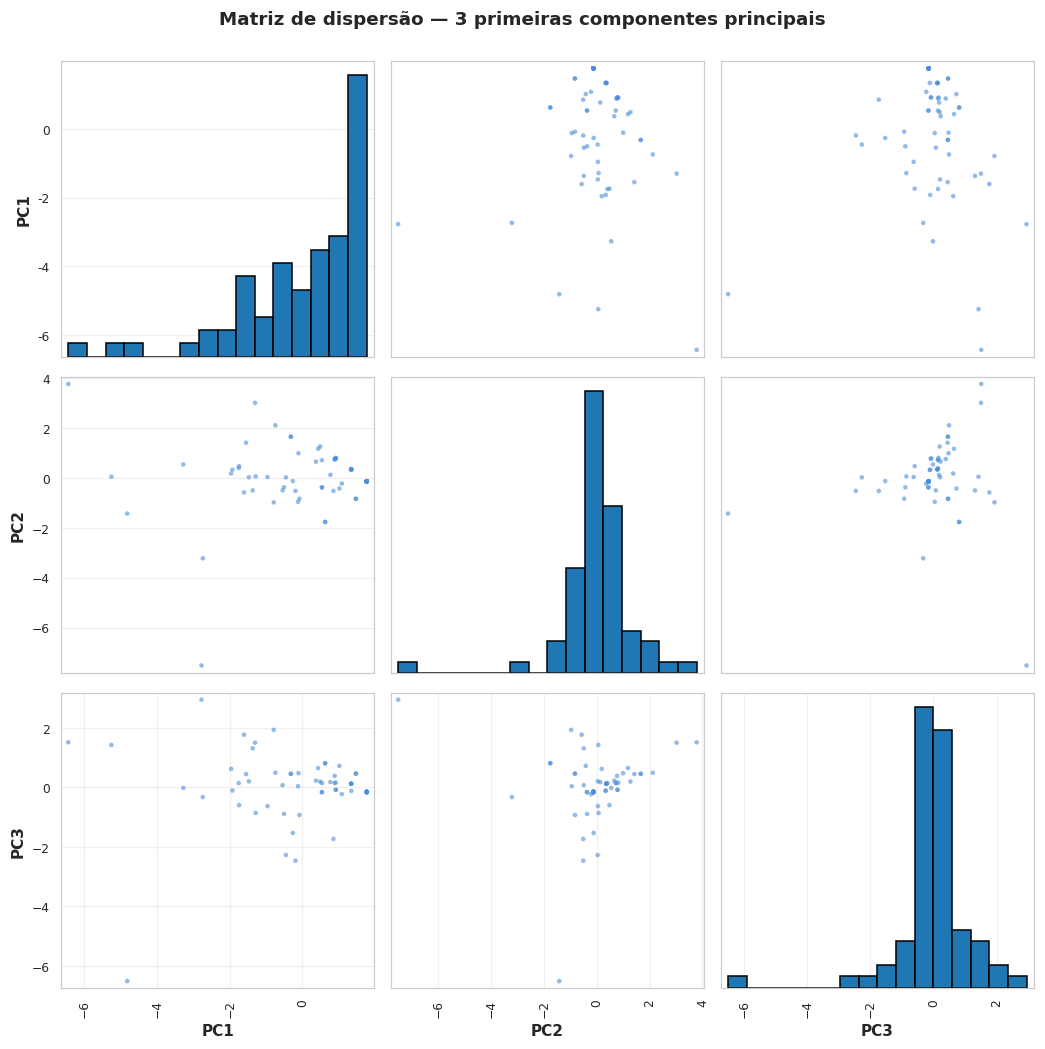
\includegraphics[width=0.8\textwidth]{figuras/matriz_dispersao_componentes.png}
    \label{fig:scatter}
    \Fonte{Elaborada pelo autor (2026).}
\end{figure}

\FloatBarrier

As projeções não revelam separação nítida entre os contextos acadêmico e industrial, nem entre as coortes: os respondentes dos dois contextos ocupam, em larga medida, a mesma região do espaço reduzido, o que é compatível com a percepção convergente sugerida pelas estatísticas descritivas. A matriz de dispersão evidencia, na diagonal, o formato das distribuições dos escores: a primeira componente concentra a maioria dos respondentes em uma faixa estreita à direita, com uma cauda à esquerda formada por poucos respondentes de avaliação geral destoante, que reaparecem como candidatos a observações atípicas na Seção \ref{sec:res-outliers}. As componentes seguintes são mais simétricas e centradas em zero. A leitura geométrica dos \textit{biplots} corrobora a estrutura de blocos: os vetores dos itens de percepção geral (desempenho, produtividade, eficácia e utilidade) agrupam-se em uma direção, os das cartas de requisitos em outra, e o vetor do contexto do mecanismo aparece destacado na terceira componente.

Esses resultados dialogam com os achados dos estudos primários. O eixo de percepção positiva geral (PC1) corresponde à avaliação uniformemente favorável reportada por \citeonline{marques2022}, \citeonline{fiori2022} e \citeonline{simoes2022usarp}. Por sua vez, os contrastes capturados por PC2 e PC3, que distinguem o bloco das cartas de requisitos, o bloco de mecanismos e os itens de percepção operacional, são consistentes com as observações qualitativas desses estudos sobre o uso diferenciado dos tipos de carta, em particular a menor utilização das cartas de prototipação e a sensibilidade da carta de contexto do mecanismo, retomadas na análise qualitativa.

\section{Detecção de Observações Atípicas}
\label{sec:res-outliers}

A Figura \ref{fig:outliers} apresenta a distância de Mahalanobis de cada respondente no espaço das cinco componentes retidas. Adotando o limiar $\chi^2_{0{,}975}(\mathrm{gl}=5) \approx 12{,}83$, cinco dos 67 respondentes (cerca de 7\%) foram sinalizados como atípicos: os respondentes de índice 3 (Acadêmico 2021-2; $D^2 = 21{,}87$), 10 (Acadêmico 2021-2; $D^2 = 13{,}22$), 34 (Acadêmico 2023-1; $D^2 = 28{,}14$), 57 (Indústria 2022; $D^2 = 44{,}77$) e 60 (Acadêmico 2025-1; $D^2 = 41{,}35$). Os casos mais extremos combinam avaliação geral mais baixa, situada na cauda à esquerda da primeira componente, com um perfil incomum de avaliação das cartas. Coerentemente com a natureza diagnóstica da análise, esses pontos não foram removidos: em uma amostra pequena, descartá-los reduziria ainda mais o poder estatístico e poderia eliminar justamente parte da variação industrial de interesse. As observações foram registradas como ressalva de robustez e como insumo para a análise qualitativa.

\begin{figure}[h!]
    \centering
    \caption{Detecção de observações atípicas pela distância de Mahalanobis}
    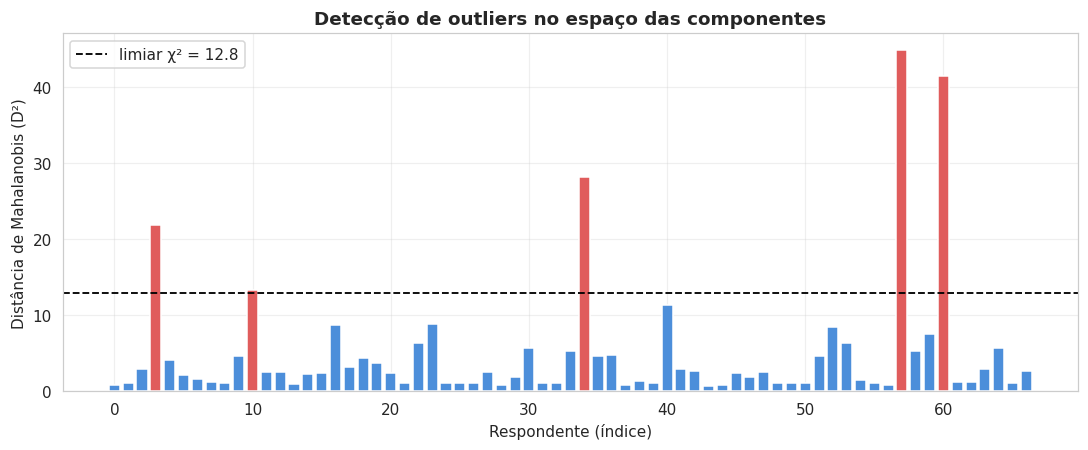
\includegraphics[width=0.9\textwidth]{figuras/outliers_mahalanobis.png}
    \label{fig:outliers}
    \Fonte{Elaborada pelo autor (2026).}
\end{figure}

\FloatBarrier

\section{Segmentação Não Supervisionada dos Perfis de Percepção}
\label{sec:res-clustering}

A Figura \ref{fig:validacao-cluster} apresenta os índices internos de validação para soluções de dois a oito grupos. O coeficiente de silhueta é máximo em $k = 2$ (0,403), e o índice de Davies-Bouldin corrobora essa leitura, de modo que se adotou a solução com dois grupos \cite{rousseeuw1987,daviesbouldin1979}. A Figura \ref{fig:kmeans} ilustra a segmentação nos planos das componentes de Kaiser, com um primeiro grupo de 17 respondentes e um segundo grupo de 50 respondentes. Para permitir a interpretação substantiva desses grupos, e não apenas sua visualização no espaço reduzido, a Tabela \ref{tab:perfil-clusters} apresenta as médias das dez variáveis originais em cada um deles, acompanhadas do contraste de Mann-Whitney item a item.

\begin{table}[h!]
\centering
\captionsetup{width=15cm}
\caption{Perfil dos grupos identificados pela segmentação k-means}
\label{tab:perfil-clusters}
\IBGEtab{}{
\begin{tabular}{lcccc}
\toprule
\textbf{Item} & \textbf{Grupo 1 (n = 17)} & \textbf{Grupo 2 (n = 50)} & \textbf{Dif.} & \textbf{p} \\
\midrule \midrule
Desempenho       & 4,06 & 4,62 & +0,56 & 0,003 \\
Produtividade    & 3,88 & 4,72 & +0,84 & $<$0,001 \\
Eficácia         & 4,00 & 4,70 & +0,70 & 0,003 \\
Utilidade        & 4,12 & 4,90 & +0,78 & $<$0,001 \\
Desc. mecanismo  & 5,18 & 5,86 & +0,68 & $<$0,001 \\
Contexto mecan.  & 5,82 & 5,92 & +0,10 & 0,837 \\
Questão requis.  & 5,24 & 5,96 & +0,72 & $<$0,001 \\
Guia requisito   & 5,12 & 5,86 & +0,74 & 0,001 \\
Questão prot.    & 5,12 & 5,86 & +0,74 & $<$0,001 \\
Guia prototip.   & 5,00 & 5,70 & +0,70 & 0,001 \\
\bottomrule
\end{tabular}
}{
\Fonte{Elaborada pelo autor (2026). Nota: Dif. = Grupo 2 menos Grupo 1; p refere-se ao teste U de Mann-Whitney entre os dois grupos.}
}
\end{table}

\FloatBarrier

O perfil dos grupos é inequívoco e tem uma leitura direta. O \textbf{Grupo 2}, majoritário, reúne 50 respondentes cuja avaliação é sistematicamente mais elevada, com médias entre 4,62 e 5,96, próximas do extremo superior das escalas; pode ser caracterizado como o perfil de \textbf{avaliação entusiástica} do método. O \textbf{Grupo 1}, minoritário, reúne 17 respondentes cuja avaliação, embora ainda positiva, é consistentemente mais contida, com médias entre 3,88 e 5,82; corresponde ao perfil de \textbf{avaliação moderada}. A diferença entre os grupos é transversal: ela se manifesta em nove dos dez itens, todos com diferença significativa, e não se concentra em um bloco específico de cartas ou em uma dimensão isolada do TAM. Em outras palavras, os dois perfis não expressam avaliações qualitativamente distintas do método, mas dois níveis de entusiasmo ao longo de um mesmo eixo de percepção positiva, exatamente o eixo capturado pela primeira componente principal.

Duas observações reforçam essa leitura. A primeira é que o único item que não distingue os grupos é justamente o contexto do mecanismo de usabilidade (5,82 contra 5,92; $p = 0{,}837$), item que satura no teto em ambos e que, por isso, não discrimina perfis de avaliação. Trata-se, do mesmo item que constitui a única diferença robusta entre coortes (Seção \ref{sec:res-comparacoes}), o que sugere que ele varia com a familiaridade com o método, e não com o nível geral de entusiasmo do respondente. A segunda é que ambos os grupos são compostos por respondentes de todas as seis coortes e dos dois contextos, conforme a Tabela \ref{tab:composicao-clusters}, o que confirma, por uma via não supervisionada, que a segmentação reflete o nível de avaliação individual e não a origem do respondente.

\begin{table}[h!]
\centering
\captionsetup{width=15cm}
\caption{Composição dos grupos por contexto e coorte}
\label{tab:composicao-clusters}
\IBGEtab{}{
\begin{tabular}{llcc}
\toprule
\textbf{Contexto} & \textbf{Coorte} & \textbf{Grupo 1} & \textbf{Grupo 2} \\
\midrule \midrule
Acadêmico & 2021-2 & 8 & 12 \\
Acadêmico & 2022-1 & 1 & 7 \\
Acadêmico & 2023-1 & 5 & 16 \\
Acadêmico & 2025-1 & 1 & 6 \\
Indústria & 2021   & 1 & 6 \\
Indústria & 2022   & 1 & 3 \\
\midrule
\multicolumn{2}{l}{\textbf{Total}} & \textbf{17} & \textbf{50} \\
\bottomrule
\end{tabular}
}{
\Fonte{Elaborada pelo autor (2026).}
}
\end{table}

\FloatBarrier

\begin{figure}[h!]
    \centering
    \caption{Seleção do número de grupos: coeficiente de silhueta e índice de Davies-Bouldin}
    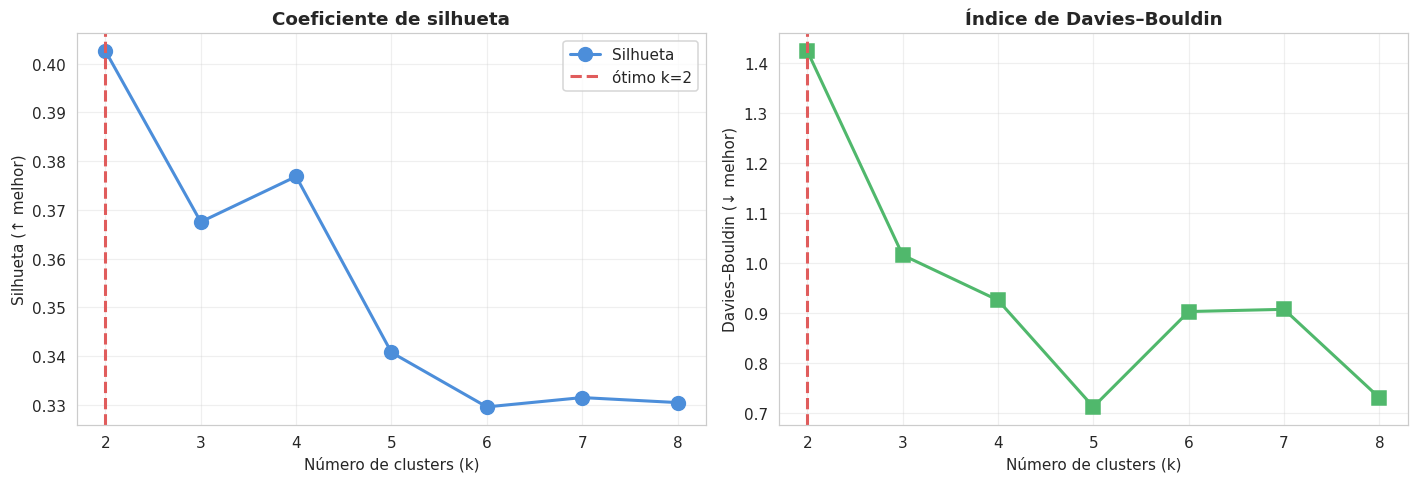
\includegraphics[width=\textwidth]{figuras/silhueta_davies_bouldin.png}
    \label{fig:validacao-cluster}
    \Fonte{Elaborada pelo autor (2026).}
\end{figure}

\begin{figure}[h!]
    \centering
    \caption{Segmentação k-means (k = 2) nos planos das componentes de Kaiser}
    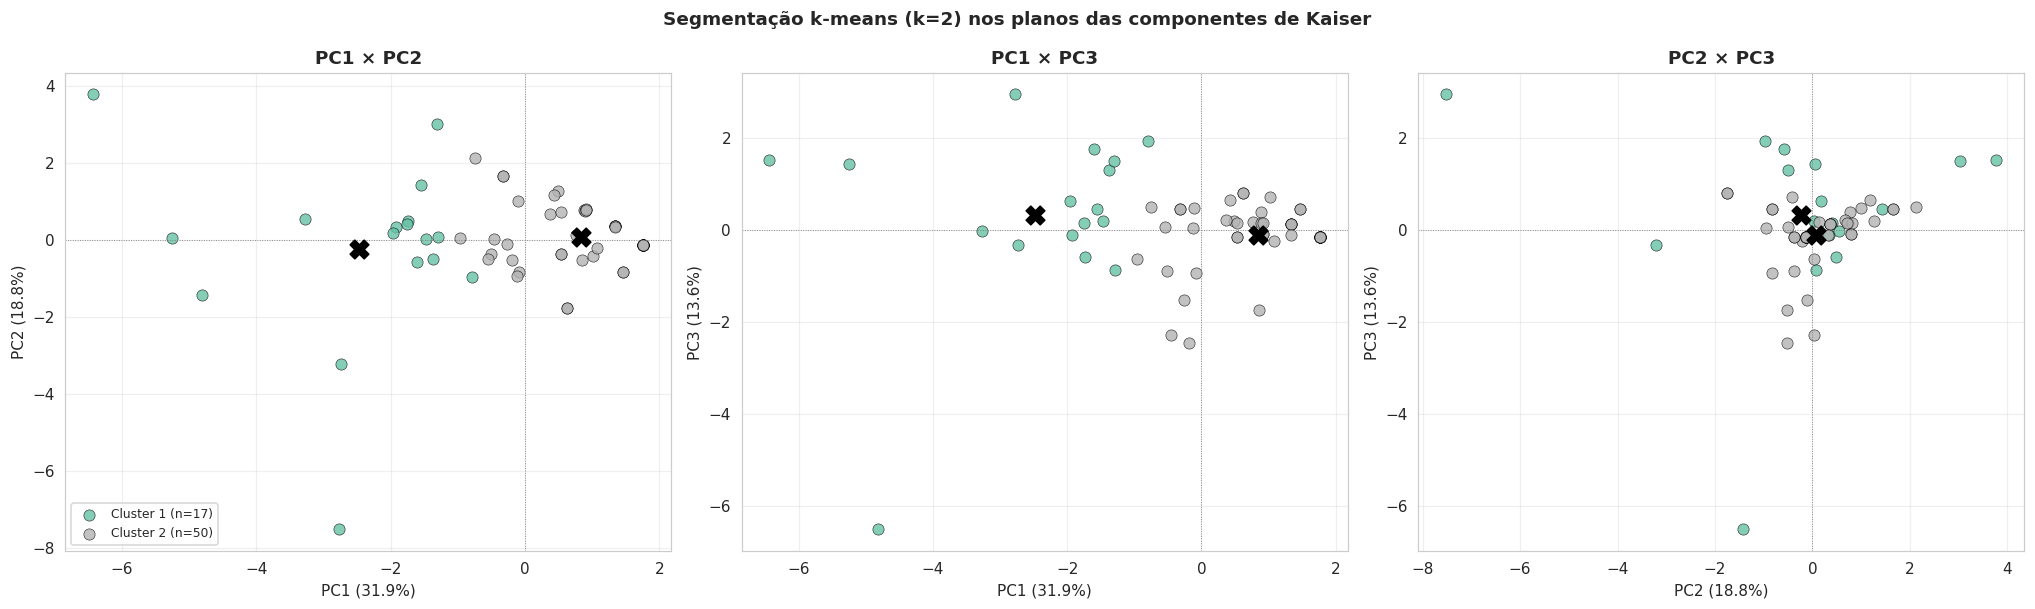
\includegraphics[width=\textwidth]{figuras/kmeans_segmentacao.png}
    \label{fig:kmeans}
    \Fonte{Elaborada pelo autor (2026).}
\end{figure}

\FloatBarrier

A Figura \ref{fig:cluster-contexto} apresenta a composição de contexto por grupo. O primeiro grupo reúne 15 respondentes acadêmicos e 2 industriais (88,2\% e 11,8\%), e o segundo, 41 acadêmicos e 9 industriais (82,0\% e 18,0\%). O teste qui-quadrado de associação entre grupo e contexto não foi significativo ($\chi^2 = 0{,}05$; $\mathrm{gl} = 1$; $p = 0{,}825$), resultado a ser interpretado com cautela em razão das contagens esperadas reduzidas. A segmentação, portanto, não é definida pelo contexto de aplicação: os dois perfis refletem essencialmente o nível geral de avaliação ao longo da primeira componente, e não a distinção entre ambientes acadêmicos e industriais. Esse achado reforça, por uma via não supervisionada, a convergência de percepção entre os cenários.

\begin{figure}[h!]
    \centering
    \caption{Composição de contexto por grupo (cluster)}
    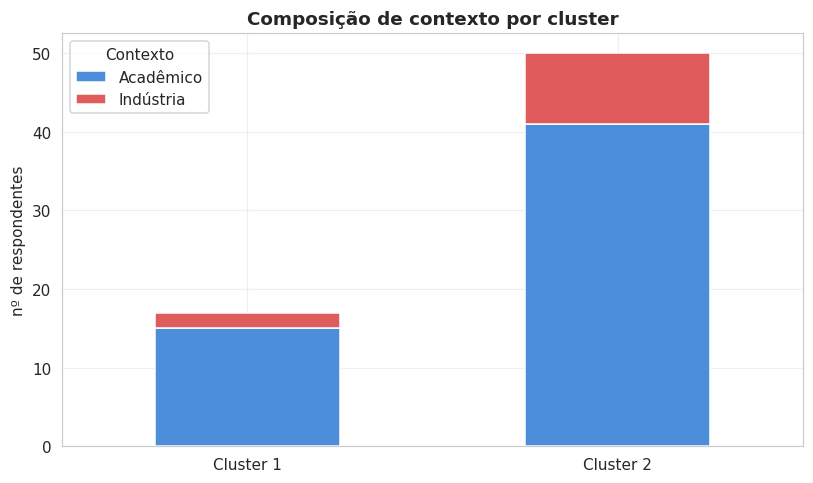
\includegraphics[width=0.7\textwidth]{figuras/composicao_contexto_cluster.png}
    \label{fig:cluster-contexto}
    \Fonte{Elaborada pelo autor (2026).}
\end{figure}

\FloatBarrier

\section{Comparações entre Grupos}
\label{sec:res-comparacoes}

As comparações foram conduzidas sobre os escores das componentes principais e, em seguida, item a item, sempre com testes não-paramétricos e correção de Holm para múltiplas comparações \cite{holm1979}. A Tabela \ref{tab:kw-componentes} apresenta o teste de Kruskal-Wallis entre as coortes, por componente, e a Tabela \ref{tab:mw-componentes} apresenta o teste de Mann-Whitney entre os contextos acadêmico e industrial, com o respectivo tamanho de efeito.

\begin{table}[h!]
\centering
\captionsetup{width=15cm}
\caption{Kruskal-Wallis entre coortes, por componente principal}
\label{tab:kw-componentes}
\IBGEtab{}{
\begin{tabular}{lcccc}
\toprule
\textbf{Componente} & \textbf{H} & \textbf{p} & \textbf{p\textsubscript{Holm}} & \textbf{Signif.} \\
\midrule \midrule
PC1 & 10,022 & 0,0746 & 0,1492 & não \\
PC2 & 12,028 & 0,0344 & 0,1032 & não \\
PC3 & 4,270  & 0,5112 & 0,5112 & não \\
\bottomrule
\end{tabular}
}{
\Fonte{Elaborada pelo autor (2026).}
}
\end{table}

\begin{table}[h!]
\centering
\captionsetup{width=15cm}
\caption{Mann-Whitney entre contextos (Acadêmico e Indústria), por componente principal}
\label{tab:mw-componentes}
\IBGEtab{}{
\begin{tabular}{lccccccc}
\toprule
\textbf{Comp.} & \textbf{Med. Acad.} & \textbf{Med. Ind.} & \textbf{U} & \textbf{p} & \textbf{r} & \textbf{p\textsubscript{Holm}} & \textbf{Signif.} \\
\midrule \midrule
PC1 & 0,53  & 0,53  & 274 & 0,5747 & 0,069 & 0,6993 & não \\
PC2 & -0,04 & -0,13 & 363 & 0,3496 & 0,115 & 0,6993 & não \\
PC3 & 0,13  & -0,15 & 417 & 0,0638 & 0,226 & 0,1914 & não \\
\bottomrule
\end{tabular}
}{
\Fonte{Elaborada pelo autor (2026).}
}
\end{table}

\FloatBarrier

A leitura componente a componente é consistente. A primeira componente, eixo de percepção positiva geral, não difere entre coortes (Kruskal-Wallis $H = 10{,}02$; $p = 0{,}075$) nem entre contextos (Mann-Whitney $U = 274$; $p = 0{,}575$), com tamanho de efeito desprezível ($r = 0{,}07$), o que indica um valor percebido alto e homogêneo entre os cenários, coerente com o efeito de teto. A segunda componente apresenta diferença bruta entre coortes ($H = 12{,}03$; $p = 0{,}034$), que deixa de ser significativa após a correção de Holm ($p_{\text{Holm}} = 0{,}103$). A terceira componente exibe o maior efeito da tabela na comparação entre contextos ($r = 0{,}23$, pequeno a moderado) e fica próxima do limiar ($p = 0{,}064$), mas também não resiste à correção ($p_{\text{Holm}} = 0{,}191$). Em síntese, após a correção de Holm, nenhuma componente difere de forma robusta entre os grupos, e os únicos sinais de contraste mostram-se frágeis frente ao controle de múltiplas comparações.

A análise item a item (Tabela \ref{tab:kw-itens}) confirma esse quadro. Nove dos dez itens são estatisticamente homogêneos entre as coortes após a correção de Holm. A produtividade chega a apresentar diferença bruta ($H = 13{,}04$; $p = 0{,}023$), mas não sobrevive à correção ($p_{\text{Holm}} = 0{,}207$). O único item que permanece significativo é o contexto do mecanismo de usabilidade (carta amarela: $H = 19{,}46$; $p_{\text{Holm}} = 0{,}016$). A análise \textit{post-hoc} de Mann-Whitney par a par, ajustada por Holm, isola as coortes responsáveis pela diferença: Indústria 2022 contra Acadêmico 2023-1 ($p_{\text{Holm}} = 0{,}019$) e Indústria 2022 contra Acadêmico 2021-2 ($p_{\text{Holm}} = 0{,}023$).

\begin{table}[h!]
\centering
\captionsetup{width=15cm}
\caption{Kruskal-Wallis entre coortes, item a item}
\label{tab:kw-itens}
\IBGEtab{}{
\begin{tabular}{lcccc}
\toprule
\textbf{Item} & \textbf{H} & \textbf{p} & \textbf{p\textsubscript{Holm}} & \textbf{Signif.} \\
\midrule \midrule
Desempenho       & 5,34  & 0,3755 & 1,0000 & não \\
Produtividade    & 13,04 & 0,0230 & 0,2068 & não \\
Eficácia         & 5,47  & 0,3615 & 1,0000 & não \\
Utilidade        & 3,59  & 0,6099 & 1,0000 & não \\
Desc. mecanismo  & 9,78  & 0,0817 & 0,6536 & não \\
Contexto mecan.  & 19,46 & 0,0016 & 0,0158 & sim \\
Questão requis.  & 1,06  & 0,9580 & 1,0000 & não \\
Guia requisito   & 8,21  & 0,1452 & 1,0000 & não \\
Questão prot.    & 2,84  & 0,7245 & 1,0000 & não \\
Guia prototip.   & 6,02  & 0,3042 & 1,0000 & não \\
\bottomrule
\end{tabular}
}{
\Fonte{Elaborada pelo autor (2026).}
}
\end{table}

\FloatBarrier

A Figura \ref{fig:medias-feature} compara as médias por item entre os contextos e ordena as diferenças. A maior diferença ocorre justamente no contexto do mecanismo, mais bem avaliado no ambiente acadêmico (5,96) do que no industrial (5,55), uma diferença de 0,42. A eficácia é o item em que a indústria supera a academia (4,82 contra 4,46, diferença de 0,35), e o desempenho é o item mais similar entre os contextos (diferença de 0,03). É importante notar que, à exceção do contexto do mecanismo, nenhuma dessas diferenças resiste ao controle de múltiplas comparações.

\begin{figure}[h!]
    \centering
    \caption{Médias por item entre contextos e diferença ordenada (Indústria menos Acadêmico)}
    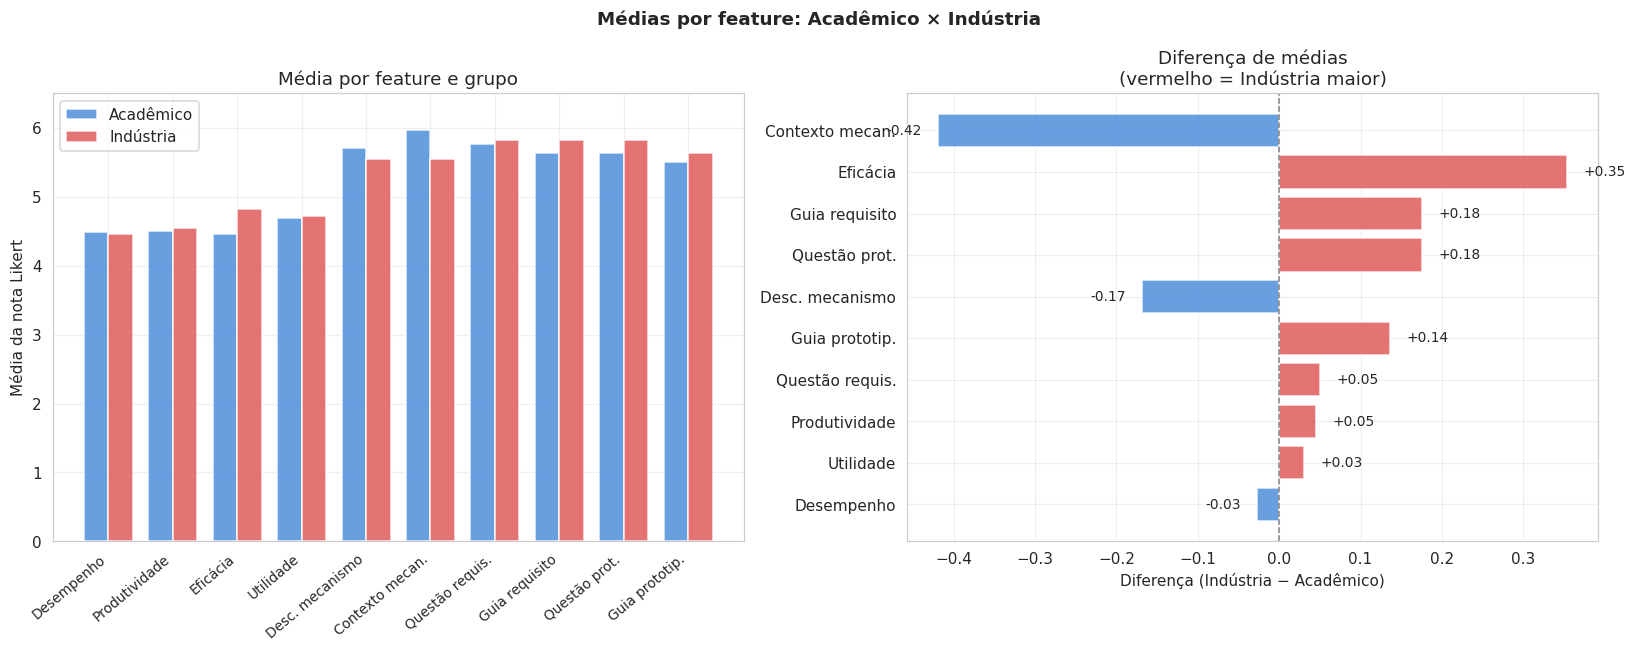
\includegraphics[width=\textwidth]{figuras/medias_feature_contexto.png}
    \label{fig:medias-feature}
    \Fonte{Elaborada pelo autor (2026).}
\end{figure}

\FloatBarrier

A diferença pontual no contexto do mecanismo de usabilidade é plausível à luz da evolução do próprio método ao longo do tempo. Como descrito por \citeonline{oliveirajr2020}, as cartas e o mecanismo de contextualização foram introduzidos e refinados após o estudo de viabilidade inicial, de modo que o grau de familiaridade e o preparo das diferentes turmas e equipes variaram entre as coortes. A coorte industrial de 2022 avalia esse item de maneira distinta das turmas acadêmicas, o que sugere que a dimensão em que os grupos mais divergem é precisamente a mais sensível à maturidade de uso do método. Esse achado dialoga diretamente com o tema qualitativo relativo ao contexto de uso e aos mecanismos, retomado na análise qualitativa.

Cabe registrar a ressalva metodológica que perpassa estas comparações. A subamostra industrial é pequena (n = 11), o que reduz o poder estatístico: a ausência de significância não comprova equivalência entre os grupos, mas apenas indica ausência de evidência de diferença \cite{field2018}. Os tamanhos de efeito foram reportados justamente para qualificar essa leitura \cite{hair2019}, e a correção de Holm foi adotada por ser uniformemente mais poderosa do que a de Bonferroni, mantendo o mesmo controle do erro do tipo I por família de comparações \cite{holm1979}. Além disso, com seis coortes de tamanhos desiguais, o número de comparações par a par é elevado e o poder é limitado, de modo que os resultados da etapa \textit{post-hoc} devem ser tratados como indicativos, e não conclusivos.

\section{Síntese dos Resultados Quantitativos}
\label{sec:res-sintese}

Os resultados quantitativos convergem para um quadro consistente. A percepção sobre o USARP é elevada e homogênea entre contextos e coortes, com forte efeito de teto em todos os itens, o que reproduz, de forma agregada, as avaliações favoráveis reportadas individualmente por \citeonline{marques2022}, \citeonline{fiori2022} e \citeonline{simoes2022usarp}. A redução de dimensionalidade revela uma primeira dimensão de percepção positiva geral, acompanhada de contrastes secundários entre os blocos de cartas (requisitos, mecanismos e prototipação) e os itens de percepção operacional. Nem a segmentação não supervisionada, que separa os respondentes por nível geral de avaliação e não por contexto, nem as comparações inferenciais, que não acusam diferenças robustas após a correção de Holm, sustentam uma distinção marcante entre ambientes acadêmicos e industriais. A única diferença que resiste ao controle estatístico, no item de contexto do mecanismo de usabilidade, aponta para a sensibilidade desse mecanismo à maturidade de uso do método, e não para uma divergência ampla de percepção.

Esses achados respondem parcialmente aos objetivos do trabalho: confirmam a percepção favorável de utilidade, produtividade e eficácia (primeiro objetivo específico) e evidenciam mais semelhanças do que diferenças entre os contextos acadêmico e industrial (terceiro objetivo específico), ao mesmo tempo em que a redução de dimensionalidade explicita as estruturas latentes associadas à aplicação do método (quarto objetivo específico). A caracterização do uso percebido dos mecanismos e a discussão das implicações práticas e limitações dependem, contudo, da leitura conjunta com as evidências qualitativas, apresentada nas seções seguintes (a partir da Seção \ref{sec:res-qualitativa}), que aprofundam os padrões de recorrência e de subutilização das cartas e contextualizam os contrastes aqui identificados.

\section{Análise Qualitativa Temática}
\label{sec:res-qualitativa}

Esta seção apresenta a análise qualitativa das respostas abertas, conduzida conforme a metodologia: codificação temática indutiva, com dicionário de termos explícito, atribuição de rótulos múltiplos e classificação de polaridade. Os trechos transcritos ao longo da seção são identificados pelo código do respondente no registro consolidado, na forma P\textit{n}, seguido do contexto e da coorte de origem, o que permite rastrear cada citação até a resposta correspondente, preservando o anonimato dos participantes. O corpus reúne as respostas abertas dos estudos que adotaram o instrumento comum, e a leitura é articulada com as evidências qualitativas reportadas nos quatro estudos primários, em especial as categorias identificadas por \citeonline{oliveirajr2020} a partir de grupo focal e as codificações por \textit{Grounded Theory} de \citeonline{fiori2022} e \citeonline{simoes2022usarp}.

\subsection{Caracterização do Corpus Qualitativo}
\label{sec:res-qual-corpus}

O corpus consolidado reúne 61 respostas abertas, distribuídas em três blocos: 34 respostas sobre características que auxiliam ou não a elicitação, 15 sobre os recursos do site de apoio e 12 sobre adaptações sugeridas para as sessões de \textit{brainstorming}. Quanto ao contexto, 47 respostas provêm do ambiente acadêmico e 14 do industrial (Tabela \ref{tab:qual-corpus}). A Figura \ref{fig:qual-corpus} apresenta a distribuição das respostas e a extensão dos relatos por contexto. As respostas do bloco de características são as mais extensas, com média de 25,3 palavras, e os relatos acadêmicos tendem a ser ligeiramente mais longos do que os industriais.

\begin{table}[h!]
\centering
\captionsetup{width=15cm}
\caption{Caracterização do corpus qualitativo por bloco}
\label{tab:qual-corpus}
\IBGEtab{}{
\begin{tabular}{lccc}
\toprule
\textbf{Bloco} & \textbf{n} & \textbf{Caracteres (média)} & \textbf{Palavras (média)} \\
\midrule \midrule
Características que auxiliam/não auxiliam & 34 & 154,3 & 25,3 \\
Recursos do site (auxiliam/não auxiliam) & 15 & 108,0 & 18,5 \\
Adaptações sugeridas no brainstorming    & 12 & 131,6 & 20,8 \\
\bottomrule
\end{tabular}
}{
\Fonte{Elaborada pelo autor (2026).}
}
\end{table}

\begin{figure}[h!]
    \centering
    \caption{Respostas por pergunta e contexto e extensão dos relatos por contexto}
    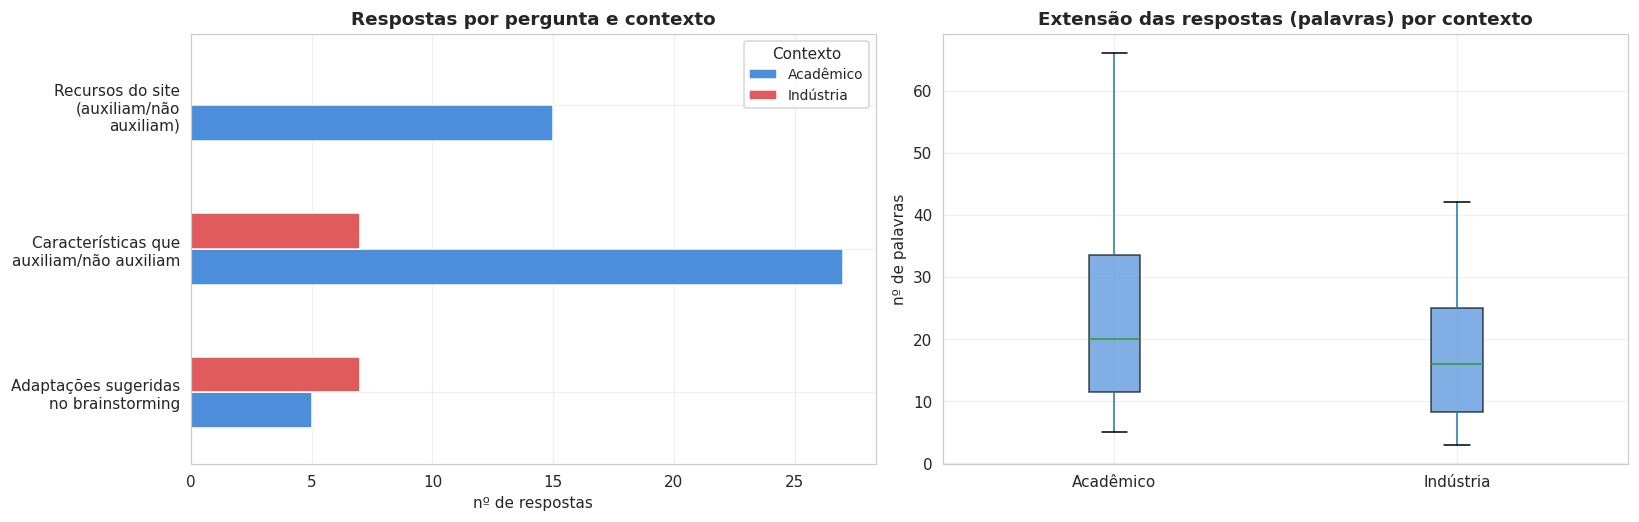
\includegraphics[width=\textwidth]{figuras/qual_respostas_pergunta_contexto.png}
    \label{fig:qual-corpus}
    \Fonte{Elaborada pelo autor (2026).}
\end{figure}

\FloatBarrier

\subsection{Características do Método que Auxiliam a Elicitação}
\label{sec:res-qual-caracteristicas}

No bloco de características (Figuras \ref{fig:qual-temas} e \ref{fig:qual-caract-adapt}), o tema dominante é, de forma destacada, o das cartas e guias como estrutura do método, com 16 menções, seguido por organização e padronização, curva de aprendizado e dificuldades, personas e \textit{user stories} e colaboração em equipe, todos com 7 menções, e por agilidade e produtividade (5), completude da elicitação (4) e contexto de uso e mecanismos (3).

A centralidade das cartas e guias confirma que os artefatos centrais do USARP, isto é, as cartas, o checklist e os guias de especificação, são percebidos como o principal motor da elicitação. Um participante da coorte acadêmica de 2025-1 sintetiza o papel de filtragem da etapa inicial e, ao mesmo tempo, a tensão de aprendizado:

\begin{citacao}
A primeira etapa da USARP é ótima para ``filtrar'' quais cartas devemos avaliar se fazem sentido com aquele requisito e ajuda muito em relação à curva de aprendizado. Algumas cartas trazem uma linguagem um pouco mais técnica de UI/UX, que por não ser da área acaba que me perco um pouco, mas se no momento do \textit{brainstorming} tiver uma pessoa do time de UI/UX fica tranquilo. (P96, Acadêmico 2025-1)
\end{citacao}

Esse relato é significativo do ponto de vista da evolução do método. A etapa de filtragem em formato de checklist resulta da evolução do método consolidada por \citeonline{marquesfiori2023}, que respondeu às dificuldades observadas por \citeonline{oliveirajr2020} no estudo de viabilidade, no qual os padrões originais (USEPs) foram considerados extensos e cansativos, motivando sua conversão em cartas. O tema da curva de aprendizado e da linguagem técnica de UI/UX, recorrente também em \citeonline{fiori2022}, mostra que essa tensão não foi eliminada, mas mitigada pela presença de perfis distintos na sessão.

A colaboração em equipe e a completude da elicitação aparecem com força nos relatos industriais, em consonância com \citeonline{marques2022}. Um participante da coorte industrial de 2021 destaca a cobertura sistemática dos requisitos:

\begin{citacao}
É interessante que todos os requisitos do sistema são lembrados de forma [organizada]; a gente tem uma ordem e um padrão a seguir para todas as \textit{user stories}. (P84, Indústria 2021)
\end{citacao}

Outro relato da mesma coorte industrial associa o detalhamento das \textit{user stories} ao debate entre profissionais de diferentes áreas, reforçando a dimensão colaborativa do método:

\begin{citacao}
A descrição de como cada \textit{feature} de uma \textit{user story} se comportará de acordo com cada ação e status do sistema. Outra característica importante é o debate e as considerações entre profissionais de áreas diferentes sobre uma determinada \textit{feature}. (P80, Indústria 2021)
\end{citacao}

A agilidade e a produtividade, por fim, aparecem associadas ao fato de as cartas oferecerem um exemplo prévio que orienta a escrita do requisito, otimizando o tempo do analista de requisitos.

\begin{figure}[h!]
    \centering
    \caption{Frequência dos temas por pergunta}
    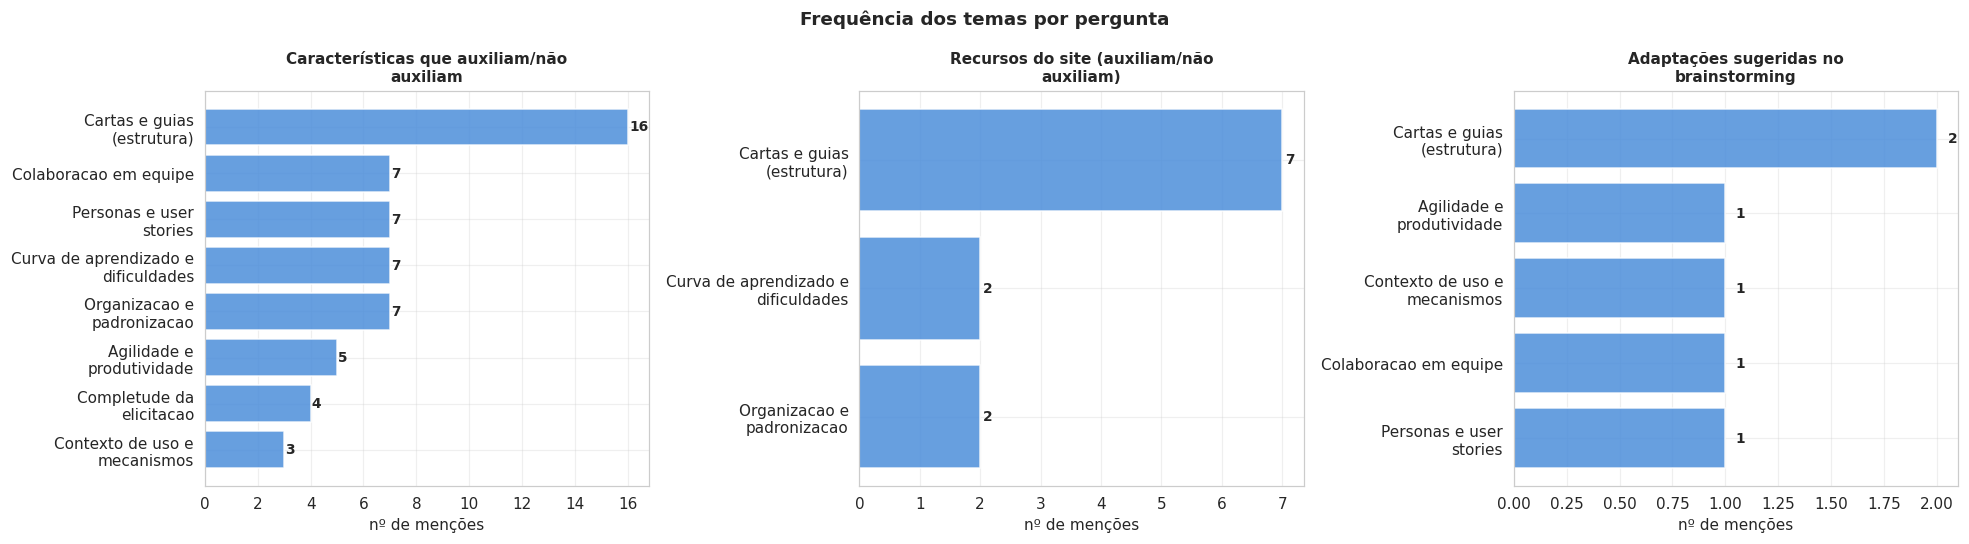
\includegraphics[width=\textwidth]{figuras/qual_temas_por_pergunta.png}
    \label{fig:qual-temas}
    \Fonte{Elaborada pelo autor (2026).}
\end{figure}

\begin{figure}[h!]
    \centering
    \caption{Categorias temáticas das características e das adaptações sugeridas}
    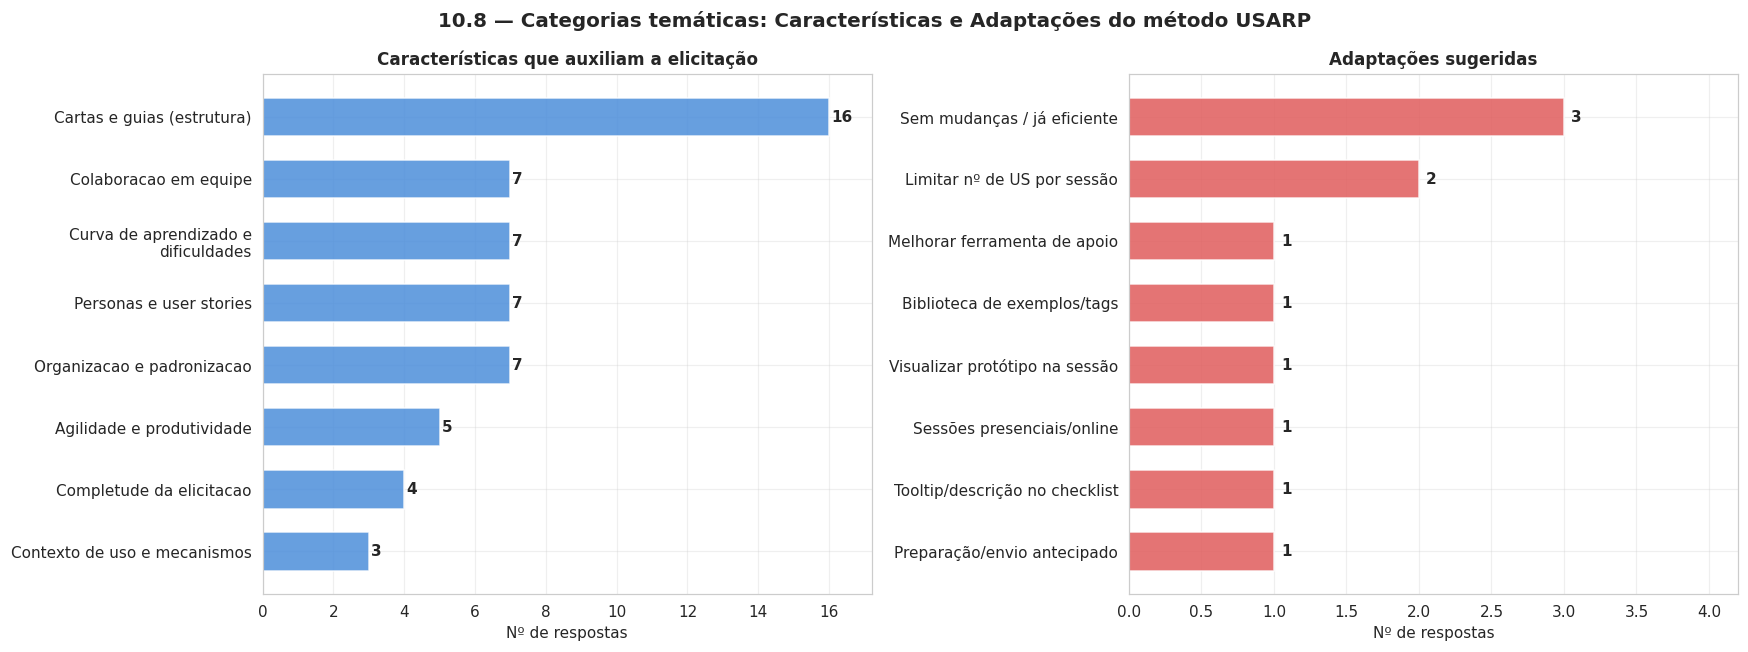
\includegraphics[width=\textwidth]{figuras/qual_categorias_caract_adapt.png}
    \label{fig:qual-caract-adapt}
    \Fonte{Elaborada pelo autor (2026).}
\end{figure}

\FloatBarrier

\subsection{Adaptações Sugeridas}
\label{sec:res-qual-adaptacoes}

As adaptações sugeridas (Figura \ref{fig:qual-caract-adapt}, à direita) são majoritariamente incrementais. A categoria mais frequente reúne participantes que não proporiam mudanças, considerando o método já eficiente (3 menções), seguida pela sugestão de limitar o número de \textit{user stories} por sessão (2 menções). As demais sugestões, com uma menção cada, concentram-se em ajustes de processo e de ferramenta: tooltips com a descrição dos mecanismos no checklist, preparação e envio prévio do material, visualização do protótipo durante a sessão, realização presencial ou online e ampliação da biblioteca de exemplos. Não há propostas de revisão estrutural do método, padrão coerente com \citeonline{marques2022}, cujos participantes igualmente não apontaram necessidade de melhorias substantivas. Um relato da coorte acadêmica de 2025-1 ilustra a percepção de eficiência:

\begin{citacao}
Creio que são bem eficientes, já que em uma sessão de cerca de 15 minutos conseguimos tirar todos os aspectos de UI/UX relacionados a um requisito. (P96, Acadêmico 2025-1)
\end{citacao}

A sugestão de limitar o número de histórias por sessão e a de incluir tooltips no checklist são especialmente informativas, pois apontam para o mesmo ponto sensível identificado na análise quantitativa: o contexto e a compreensão dos mecanismos.

\subsection{Recursos do Site de Apoio}
\label{sec:res-qual-site}

Dos 61 relatos, 15 referem-se ao site de apoio (Figura \ref{fig:qual-site}). Os aspectos positivos predominam: o material para download das cartas em PDF (7 menções), o material didático e a explicação dos conceitos (6), a interface e a organização (4) e o apoio ao \textit{brainstorming} (3). As limitações são pontuais e dizem respeito à usabilidade da ferramenta: navegação por vezes confusa (2), dúvidas não totalmente esclarecidas (2), ausência de conteúdo prático em vídeo (1) e carregamento das cartas (1). Um relato da coorte acadêmica de 2021-2 sintetiza o valor didático do recurso e, ao mesmo tempo, uma limitação de navegação:

\begin{citacao}
Gostei bastante do site; no começo fiquei muito confusa e perdida quanto ao método e às cartas, mas as explicações presentes no site ajudaram, e muito, a conseguir organizar as reuniões de maneira mais efetiva. (P25, Acadêmico 2021-2)
\end{citacao}

Outro participante da mesma coorte sugere conteúdo prático adicional:

\begin{citacao}
Todo o conteúdo do site ajudou o grupo a saber como fazer a elicitação de requisitos usando o método USARP, mas eu achei que faltou informação prática; seria bom algum link para ver um vídeo com pessoas fazendo a elicitação com esse método, mostrando o objetivo do tipo de cada carta. (P6, Acadêmico 2021-2)
\end{citacao}

\begin{figure}[h!]
    \centering
    \caption{Categorias temáticas dos recursos do site: aspectos positivos e limitações}
    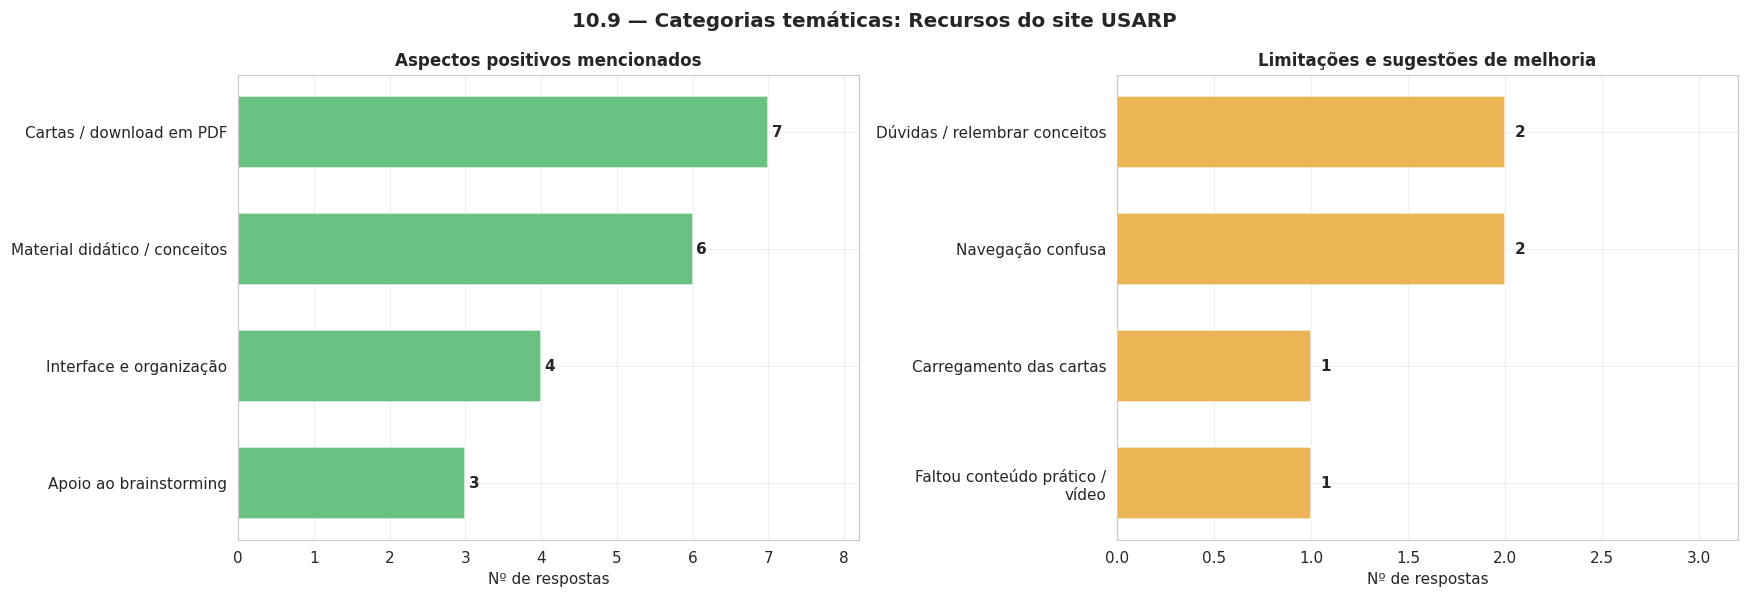
\includegraphics[width=\textwidth]{figuras/qual_categorias_site.png}
    \label{fig:qual-site}
    \Fonte{Elaborada pelo autor (2026).}
\end{figure}

\FloatBarrier

\subsection{Polaridade e Tom das Respostas}
\label{sec:res-qual-polaridade}

A classificação de polaridade (Figura \ref{fig:qual-polaridade}) indica predomínio de respostas positivas (27), seguidas de respostas mistas (16) e neutras (16), com apenas 2 respostas negativas. A distribuição por bloco é coerente com a natureza de cada pergunta: o bloco de características concentra 79\% de respostas positivas ou mistas e o do site, 87\%, enquanto o bloco de adaptações é majoritariamente neutro, o que é esperado, dado que reúne sugestões e não avaliações. Os termos de conteúdo mais frequentes (Figura \ref{fig:qual-termos}) reforçam o foco nos artefatos do método: ``cartas'' (24 ocorrências), ``requisitos'' (13), ``site'' (11) e ``método'' (10) lideram a contagem.

\begin{figure}[h!]
    \centering
    \caption{Polaridade das respostas por pergunta e por contexto}
    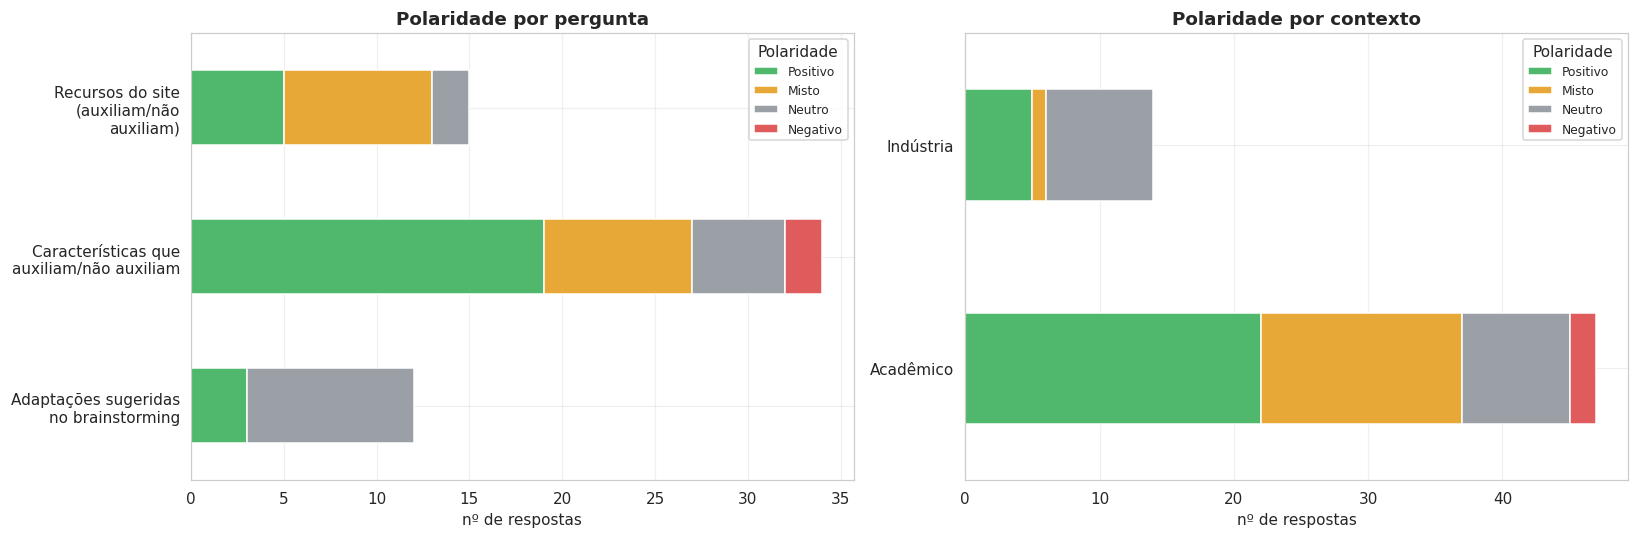
\includegraphics[width=\textwidth]{figuras/qual_polaridade.png}
    \label{fig:qual-polaridade}
    \Fonte{Elaborada pelo autor (2026).}
\end{figure}

\begin{figure}[h!]
    \centering
    \caption{Termos de conteúdo mais frequentes nas respostas abertas}
    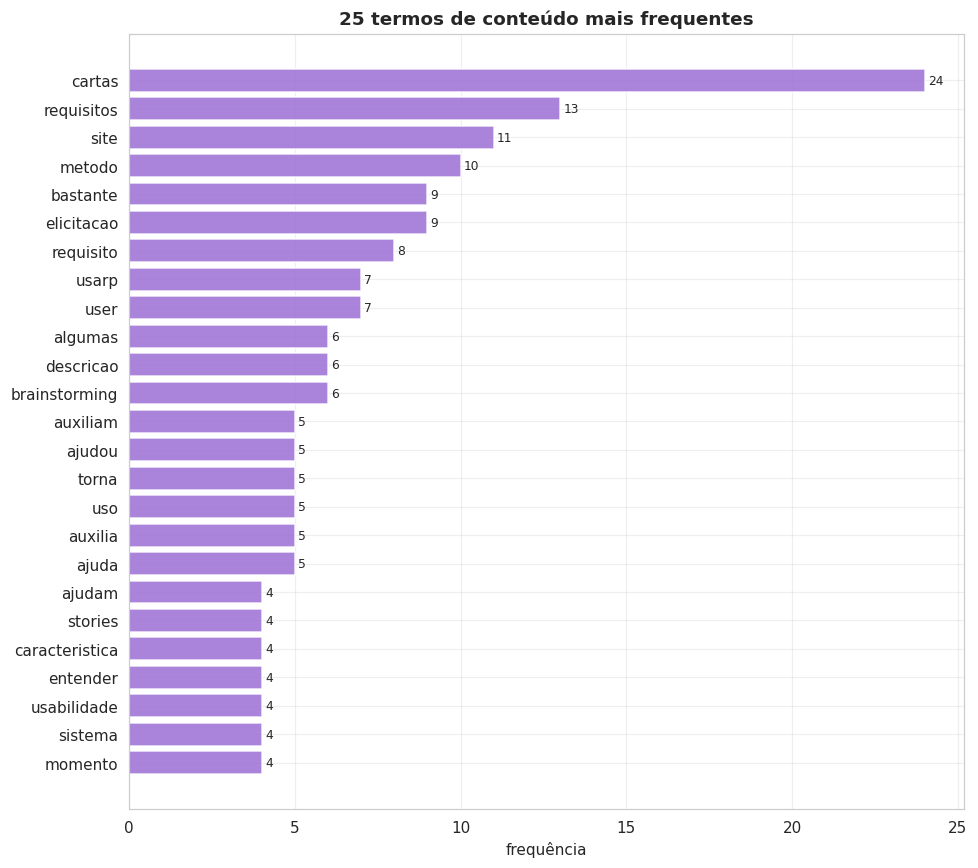
\includegraphics[width=0.75\textwidth]{figuras/qual_termos_frequentes.png}
    \label{fig:qual-termos}
    \Fonte{Elaborada pelo autor (2026).}
\end{figure}

\FloatBarrier

\subsection{Síntese Qualitativa e Relação com os Estudos Primários}
\label{sec:res-qual-sintese}

A Tabela \ref{tab:qual-sintese} e a Figura \ref{fig:qual-dominante} consolidam a leitura dos três blocos. Antes delas, a Tabela \ref{tab:mencoes-tema} apresenta, de forma sistematizada, a contagem de menções por tema, discriminada por bloco de pergunta e por contexto, complementando a leitura gráfica da Figura \ref{fig:qual-temas}.
\begin{table}[h!]
\centering
\captionsetup{width=15cm}
\caption{Menções por tema, segundo o bloco de pergunta e o contexto}
\label{tab:mencoes-tema}
\IBGEtab{}{
\resizebox{\textwidth}{!}{%
\begin{tabular}{lcccccc}
\toprule
\textbf{Tema} & \textbf{Características} & \textbf{Site} & \textbf{Adaptações} & \textbf{Total} & \textbf{Acadêmico} & \textbf{Indústria} \\
\midrule \midrule
Cartas e guias (estrutura)          & 16 & 7 & 2 & 25 & 25 & 0 \\
Organização e padronização          & 7  & 2 & 0 & 9  & 8  & 1 \\
Curva de aprendizado e dificuldades & 7  & 2 & 0 & 9  & 9  & 0 \\
Colaboração em equipe               & 7  & 0 & 1 & 8  & 4  & 4 \\
Personas e user stories             & 7  & 0 & 1 & 8  & 5  & 3 \\
Agilidade e produtividade           & 5  & 0 & 1 & 6  & 4  & 2 \\
Completude da elicitação            & 4  & 0 & 0 & 4  & 2  & 2 \\
Contexto de uso e mecanismos        & 3  & 0 & 1 & 4  & 4  & 0 \\
\midrule
\textbf{Total de atribuições}       & \textbf{56} & \textbf{11} & \textbf{6} & \textbf{73} & \textbf{61} & \textbf{12} \\
\bottomrule
\end{tabular}%
}
}{
\Fonte{Elaborada pelo autor (2026). Nota: como a codificação admite rótulos múltiplos, o total de atribuições excede o número de respostas (61).}
}
\end{table}

\FloatBarrier

O bloco de características é dominado pelo tema das cartas e guias; o de adaptações, pela ausência de mudanças propostas; e o do site, pela valoração positiva do material das cartas, cuja principal limitação é a navegação por vezes confusa. Em conjunto, os achados qualitativos desenham um quadro consistente com as evidências dos quatro estudos primários. A percepção de estrutura, organização e completude proporcionada pelas cartas reproduz os relatos de \citeonline{marques2022} e \citeonline{fiori2022}; a dimensão colaborativa ecoa o uso do método em sessões com profissionais de diferentes papéis descrito por \citeonline{marques2022}; e as tensões relativas à curva de aprendizado e ao volume e à linguagem das cartas remontam às dificuldades originalmente registradas por \citeonline{oliveirajr2020} e reiteradas por \citeonline{fiori2022} e \citeonline{simoes2022usarp}.

Um ponto merece destaque pela convergência entre os estudos: a subutilização das cartas de prototipação. \citeonline{simoes2022usarp} observam que os aspectos de prototipação foram pouco explorados, e \citeonline{marquesfiori2023}, na análise documental dos trabalhos produzidos, identificaram que a carta de especificação de prototipação foi percebida como um obstáculo por parte dos participantes e que alguns mecanismos, como os de preferências e de área de objetos pessoais, foram subutilizados. O mesmo padrão emerge na presente síntese, tanto qualitativamente, pela menor presença do tema, quanto quantitativamente, já que o guia de prototipação apresenta a menor média entre os itens de cartas (5,52). Esse alinhamento entre os relatos discursivos, a análise de artefatos de \citeonline{marquesfiori2023} e as medidas numéricas fortalece a robustez do achado.

\begin{table}[h!]
\centering
\captionsetup{width=15cm}
\caption{Síntese qualitativa por bloco}
\label{tab:qual-sintese}
\IBGEtab{}{
\begin{tabular}{lccc}
\toprule
\textbf{Bloco} & \textbf{n} & \textbf{Categoria dominante} & \textbf{\% positivo/misto} \\
\midrule \midrule
Características  & 34 & Cartas e guias (estrutura) (16) & 79\% \\
Adaptações      & 12 & Sem mudanças / já eficiente (3) & 25\% \\
Site (positivo) & 15 & Cartas / download em PDF (7)    & 87\% \\
\bottomrule
\end{tabular}
}{
\Fonte{Elaborada pelo autor (2026).}
}
\end{table}

\begin{figure}[h!]
    \centering
    \caption{Categoria dominante por bloco qualitativo}
    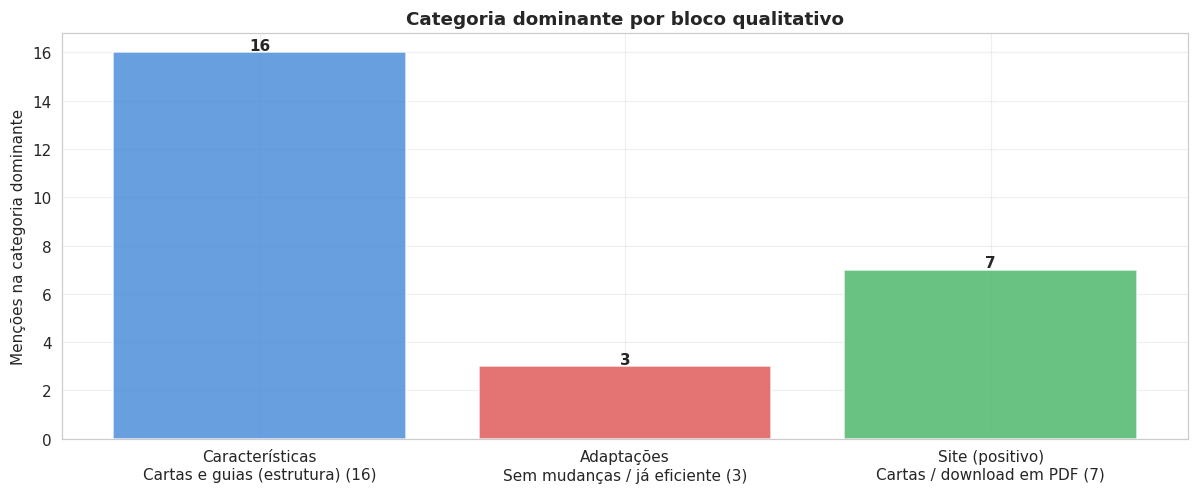
\includegraphics[width=0.8\textwidth]{figuras/qual_categoria_dominante_bloco.png}
    \label{fig:qual-dominante}
    \Fonte{Elaborada pelo autor (2026).}
\end{figure}

\FloatBarrier

\section{Discussão Integrada dos Resultados}
\label{sec:res-discussao}

Esta seção articula as evidências quantitativas e qualitativas e as relaciona aos objetivos do trabalho. A Figura \ref{fig:sintese-integrada} confronta, lado a lado, as médias dos itens do levantamento e a frequência dos temas qualitativos.

\begin{figure}[h!]
    \centering
    \caption{Síntese integrada: médias do levantamento e frequência dos temas qualitativos}
    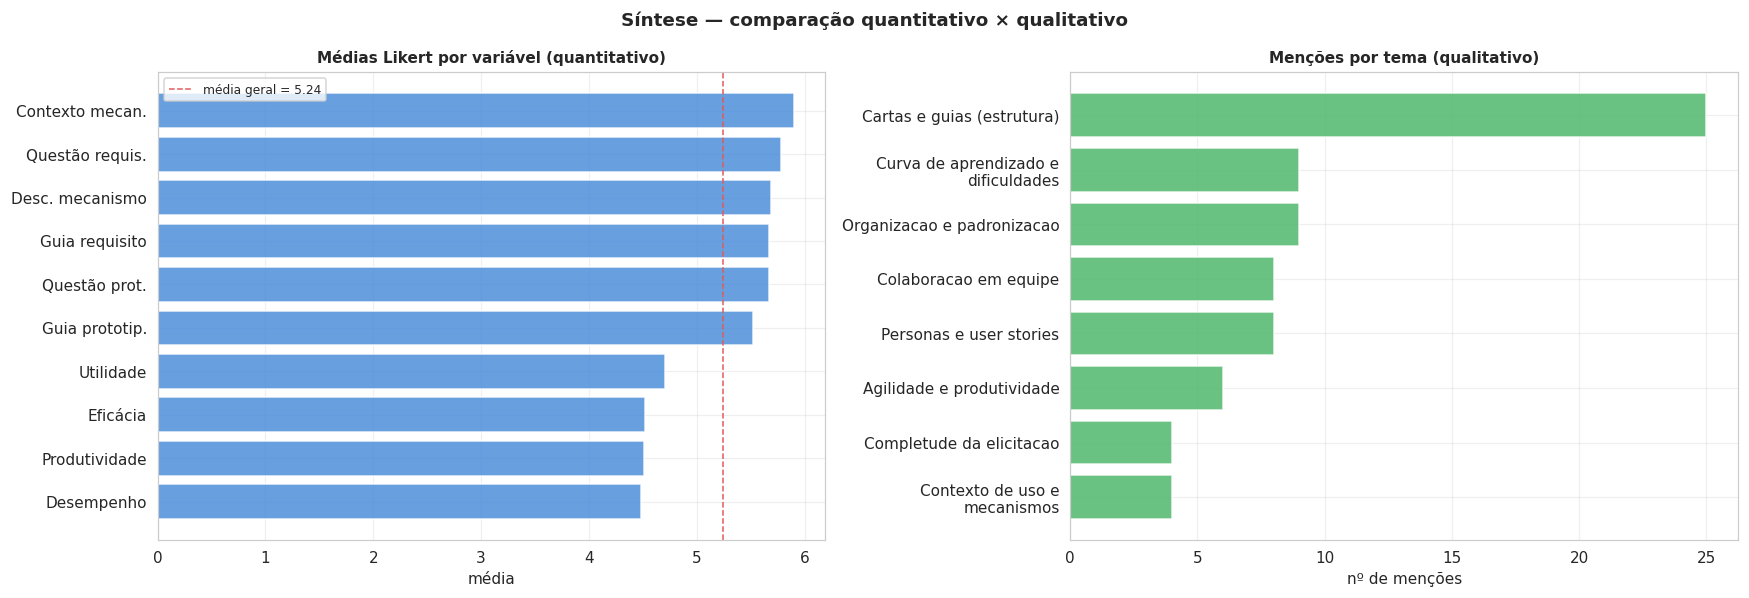
\includegraphics[width=\textwidth]{figuras/sintese_quanti_quali.png}
    \label{fig:sintese-integrada}
    \Fonte{Elaborada pelo autor (2026).}
\end{figure}

\FloatBarrier

A leitura integrada revela forte coerência entre os dois conjuntos de evidência. Os itens com maiores médias no levantamento são os relativos ao conteúdo das cartas, com destaque para o contexto do mecanismo (5,90), a questão de requisitos (5,78) e a descrição do mecanismo (5,69), e o tema mais citado qualitativamente é justamente o das cartas e guias como estrutura do método, com 25 menções no total. A convergência se estende às tensões: as dificuldades apontadas nos relatos, isto é, a curva de aprendizado, a quantidade de cartas e a linguagem técnica de UI/UX, ajudam a explicar por que os itens de percepção operacional do TAM (desempenho, 4,48; produtividade, 4,51; eficácia, 4,52), embora positivos, recebem médias inferiores às dos itens de conteúdo das cartas. Em outras palavras, o conteúdo das cartas é altamente valorizado, ao passo que a experiência operacional de aplicá-las ainda esbarra na curva de aprendizado.

Essa convergência também esclarece o único contraste estatístico robusto identificado na análise quantitativa. O item de contexto do mecanismo de usabilidade, no qual a coorte industrial de 2022 diverge das turmas acadêmicas, corresponde, no plano qualitativo, ao tema de contexto de uso e mecanismos e à própria sugestão de incluir, no checklist, uma descrição de cada mecanismo. Trata-se, portanto, da dimensão mais sensível à maturidade de uso e ao grau de familiaridade com o método, o que é compatível com a sua trajetória de evolução, das USEPs densas de \citeonline{oliveirajr2020} para as cartas e a etapa de filtragem em checklist propostas por \citeonline{marquesfiori2023}. Cabe notar que a dificuldade de seleção e de compreensão das cartas é justamente a motivação central do \textit{checklist} e do quadro propostos por \citeonline{marquesfiori2023}, o que reforça a leitura de que o item mais sensível da síntese coincide com o ponto que a própria evolução do método buscou endereçar. A leitura conjunta, na qual o conteúdo qualitativo ajuda a explicar os padrões numéricos, reforça a validade dos achados pela convergência entre as evidências \cite{braunclarke2006}.

À luz dos objetivos específicos, os resultados permitem as seguintes conclusões parciais. Quanto ao primeiro objetivo, a percepção de utilidade, produtividade e eficácia mostrou-se elevada e homogênea entre contextos, ainda que os itens operacionais recebam médias um pouco inferiores às do conteúdo das cartas. Quanto ao segundo objetivo, a caracterização do uso percebido dos mecanismos evidenciou as cartas e os guias como o principal motor da elicitação e revelou a subutilização das cartas de prototipação, padrão convergente entre os relatos e as médias. Quanto ao terceiro objetivo, observaram-se mais semelhanças do que diferenças entre os contextos acadêmico e industrial, com a única divergência robusta restrita ao item de contexto do mecanismo. Quanto ao quarto objetivo, a análise de componentes principais explicitou as estruturas latentes, com uma dimensão de percepção positiva geral e contrastes secundários entre os blocos de cartas e os itens de percepção operacional. Por fim, as implicações práticas e as limitações, objeto do quinto objetivo, são aprofundadas no capítulo de considerações finais.